% Working manuscript: includes measured x86 detector and latency pilot results.
\documentclass{ieeeaccess}
\usepackage{cite}
\usepackage{amsmath,amssymb,amsfonts}
\usepackage{algorithmic}
\usepackage{graphicx}
\usepackage{textcomp}
\usepackage{array}
\usepackage{booktabs}
\usepackage{multirow}
\usepackage{float}
% The IEEE Access class uses the caption package's standard caption format.
\makeatletter
\def\caption@documentclass{standard}
\makeatother
\usepackage{caption}
\usepackage{hyperref}
\hypersetup{hidelinks}
\usepackage{url}
\makeatletter
% Older IEEE Access class files do not initialize optional publication fields.
\providecommand{\@doi}{}
\providecommand{\@history}{}
\def\@IEEEBIOskipN{1\baselineskip}
% Standard figure environments do not set the class's optional width macro.
\providecommand{\xfigwd}{0pt}
\setlength{\@dblfptop}{0pt}
\makeatother
\setlength{\textfloatsep}{9pt plus 2pt minus 2pt}
\setlength{\dbltextfloatsep}{9pt plus 2pt minus 2pt}
\setlength{\floatsep}{7pt plus 2pt minus 2pt}
\setlength{\intextsep}{8pt plus 2pt minus 2pt}
% The manuscript uses regular-weight text throughout.
\renewcommand{\textbf}[1]{#1}
\let\bfseries\mdseries
\raggedbottom
\def\BibTeX{{\rm B\kern-.05em{\sc i\kern-.025em b}\kern-.08em
    T\kern-.1667em\lower.7ex\hbox{E}\kern-.125emX}}
\begin{document}

\title{A Rust Security Posture and Anomaly Detection Prototype for K3s Edge Nodes}

\author{
\uppercase{Semunyu Aloyzious}\authorrefmark{1},
\uppercase{Odoi Stephen}\authorrefmark{1}
}

\address[1]{Department of Computer Science, Makerere University, Kampala, Uganda (e-mail: semunyu.aloyzious@students.mak.ac.ug; odoi.stephen@students.mak.ac.ug)}

\tfootnote{This work was supported in part by Makerere University under the Graduate Research Fellowship Program.}

\markboth
{Semunyu and Odoi: Rust Posture and Anomaly Detection for K3s Edge Nodes}
{Semunyu and Odoi: Rust Posture and Anomaly Detection for K3s Edge Nodes}


\begin{abstract}
Healthcare registries in resource-constrained settings need security monitoring suited to edge computing. We present Lightweight Dynamic Posture and Anomaly Detection (LDPAD), a Rust prototype for posture and anomaly assessment. Its command-line program and a labelled synthetic detector driver were executed inside a test pod managed by a single-node K3s cluster on an Ubuntu laptop virtual machine (VM).

\par\smallskip
The K3s-pod driver, configured for 30 seeds, produced 15,000 synthetic samples. It matched 300/300 labelled one-tick CPU spikes and alerted on 198/13,800 post-warm-up non-spike ticks (1.43\%); non-spike ticks comprised 198/498 alert-bearing ticks (39.8\%). An earlier x86\_64 host run of the same seeded design had the same aggregate counts; the rerun is not an independent attack study. The host's exact 95\% intervals were 98.78--100.00\% for spike matches and 1.24--1.65\% for non-spike alert ticks, assuming independent observations. Elapsed detection delay and alerts per node-day were not measured.

\par\smallskip
In a separate fusion simulation, a guarded design reached Strict three simulated seconds after sustained high runtime risk began, but a three-second nuisance pulse also triggered Strict and two boundary reversals. A separate laptop-VM loopback pilot had a P99 of 29.812~ms and a 95\% upper bound of 56.075~ms at 10 requests/s. The completed pod run demonstrates K3s-hosted execution; continuous cluster monitoring, real attacks, the admission-to-log path and physical edge devices remain to be evaluated.
\end{abstract}

\begin{keywords}
Cloud Security, Security Posture, Anomaly Detection, Rust, K3s, Edge Computing, Healthcare Registries
\end{keywords}

\titlepgskip=-15pt

\maketitle
\section{Introduction}
\label{sec:introduction}

The rapid digitization of healthcare systems has fundamentally transformed patient care delivery across the globe. Cloud-based Electronic Health Records (EHRs), telemedicine platforms, and Internet of Medical Things (IoMT) devices have become essential infrastructure for modern healthcare delivery~\cite{b1,b2}. Cloud computing has emerged as the backbone of this transformation, enabling scalable storage solutions, remote consultations, interoperable EHRs, and real-time IoMT analytics.

However, this digital transformation has introduced critical security vulnerabilities that expose sensitive patient information to a growing array of cyber threats. Cloud security risks include misconfigurations, overly permissive access policies, publicly exposed storage buckets, non-compliant network policies, and improperly secured container runtimes. Ransomware attacks, phishing campaigns, malware infections, unauthorized access, and data breaches have become increasingly sophisticated, targeting the confidentiality, integrity, and availability of healthcare data.

The challenge is particularly acute in low-resource healthcare settings---rural clinics, developing-region hospitals, and disaster-response scenarios---where computing resources, connectivity, IT expertise and reliable power can be limited~\cite{b3,b4}. In such environments, assumptions of continuous cloud connectivity and abundant compute resources may lead to compromised security posture and delayed anomaly detection.

\subsection{Problem Statement}
\label{subsec:problem}

Cloud-based healthcare registries in low-resource environments face a multi-objective design challenge. This conflict manifests across three competing objectives:

{Security Posture Rigor:} Healthcare organizations must maintain compliance with regulatory frameworks such as the Ugandan Data Protection and Privacy Act (DPPA), the Health Insurance Portability and Accountability Act (HIPAA), and the General Data Protection Regulation (GDPR). Applicable obligations for privacy, security and incident reporting depend on the deployment and the jurisdiction. Achieving these requirements demands continuous security posture assessment, zero-trust enforcement, and runtime threat detection---each imposing significant computational and bandwidth costs.

{Resource Efficiency:} Healthcare deployments in low-resource settings may have limited memory and central processing unit (CPU) capacity, intermittent power and constrained network bandwidth~\cite{b3,b11}. These constraints can conflict with the resource overhead imposed by modern security mechanisms.

{Clinical Responsiveness:} Real-time anomaly detection must not disrupt patient care. Clinicians require immediate access to patient records, and any security mechanism that introduces latency spikes---particularly 99th-percentile (P99) latency spikes---risks operational failure in time-sensitive scenarios~\cite{b14,b15}.

The research challenge is to balance these objectives while configurations, threat information, and workload patterns change. The available literature and tool comparisons do not yet establish that any design is unique, superior, or suitable for a particular resource envelope.

Configuration scanning, runtime monitoring and policy enforcement inspect different events. Whether combining their findings improves detection or operational cost must be established against named tools using a common workload; it cannot be concluded from the present component experiments.

\subsection{Research Questions}
\label{subsec:rq}

The following questions guide the study. The present experiments answer them only in part: they evaluate Rust components with synthetic inputs, including execution in a K3s test pod, a simulated fusion candidate and a separate laptop-VM loopback pilot. Continuous K3s monitoring and physical edge-node performance remain untested.

\begin{itemize}
\item \textbf{RQ1:} What are the minimum security controls required for effective security posture under severe resource constraints? H1a tests detection effectiveness; establishing a minimum also requires an ablation.
\item {RQ2:} How can dynamic, continuous posture assessment be performed in a resource-limited environment, and what are its measured CPU and memory costs? (H1b--H1d)
\item {RQ3:} How can runtime anomaly detection be integrated with dynamic posture assessment without excessive overhead? (H1a, H1c, H1d, H1e)
\item {RQ4:} How can detection integrity be maintained during network partitions in disconnected clinical environments? (H1a and H1f)
\item {RQ5:} What computational overhead do different security mechanisms impose on constrained devices? (H1b--H1d; component attribution requires an ablation)
\end{itemize}

\subsection{Contribution Statement}
\label{subsec:contribution}

This paper makes four contributions:

\begin{enumerate}
\item {Rust prototype components} for posture checking, drift detection, anomaly detection and weighted risk scoring, exercised with synthetic inputs.
\item {A labelled detector study} reporting spike matches and clean-tick alerts for 30 seeded synthetic runs, with a repeated execution inside a K3s test pod.
\item {A guarded fusion study} comparing three scoring approaches on fixed, design-labelled virtual-time scenarios.
\item {A laptop-VM latency pilot} measuring a separate Rust, Regorus and SQLite loopback path using synthetic requests.
\end{enumerate}

\section{Literature Review and Evidence Status}
\label{sec:gapanalysis}

This section describes the reported search, the reference inventory and the status of the evidence matrix.

\subsection{Search and Screening Protocol}
\label{subsec:prisma}

The reported search date is 15 August 2026, using IEEE Xplore, ACM Digital Library, Scopus and ScienceDirect. The generic Boolean string below targets titles, abstracts and keywords. Database-specific syntax, execution logs and result exports are unavailable for independent verification:

\noindent\begin{minipage}{\columnwidth}
\footnotesize
\begin{verbatim}
("healthcare" OR "medical" OR "clinical")
AND ("cloud" OR "edge" OR "kubernetes"
     OR "K3s")
AND ("security" OR "posture" OR "anomaly"
     OR "drift" OR "intrusion")
AND ("resource-constrained" OR
     "low-resource" OR "edge computing")
\end{verbatim}
\end{minipage}

Here \emph{posture} is one alternative within the broader security block. The reported counts are 127 records, 38 duplicates, 69 records after title-and-abstract screening and 25 retained publications, with 44 full-text exclusions including 10 on publication date. Independent screening of 20\% of records and $\kappa=0.81$ were also reported, but the sampling frame, number of records, selections and adjudications are unavailable. These counts and screening claims cannot be independently verified. Figure~\ref{fig:prisma_reported} presents the available counts using the structure of Preferred Reporting Items for Systematic Reviews and Meta-Analyses (PRISMA) 2020~\cite{b_prisma}; retrieval stages and per-database counts require the original records.

\begin{figure*}[t]
\centering
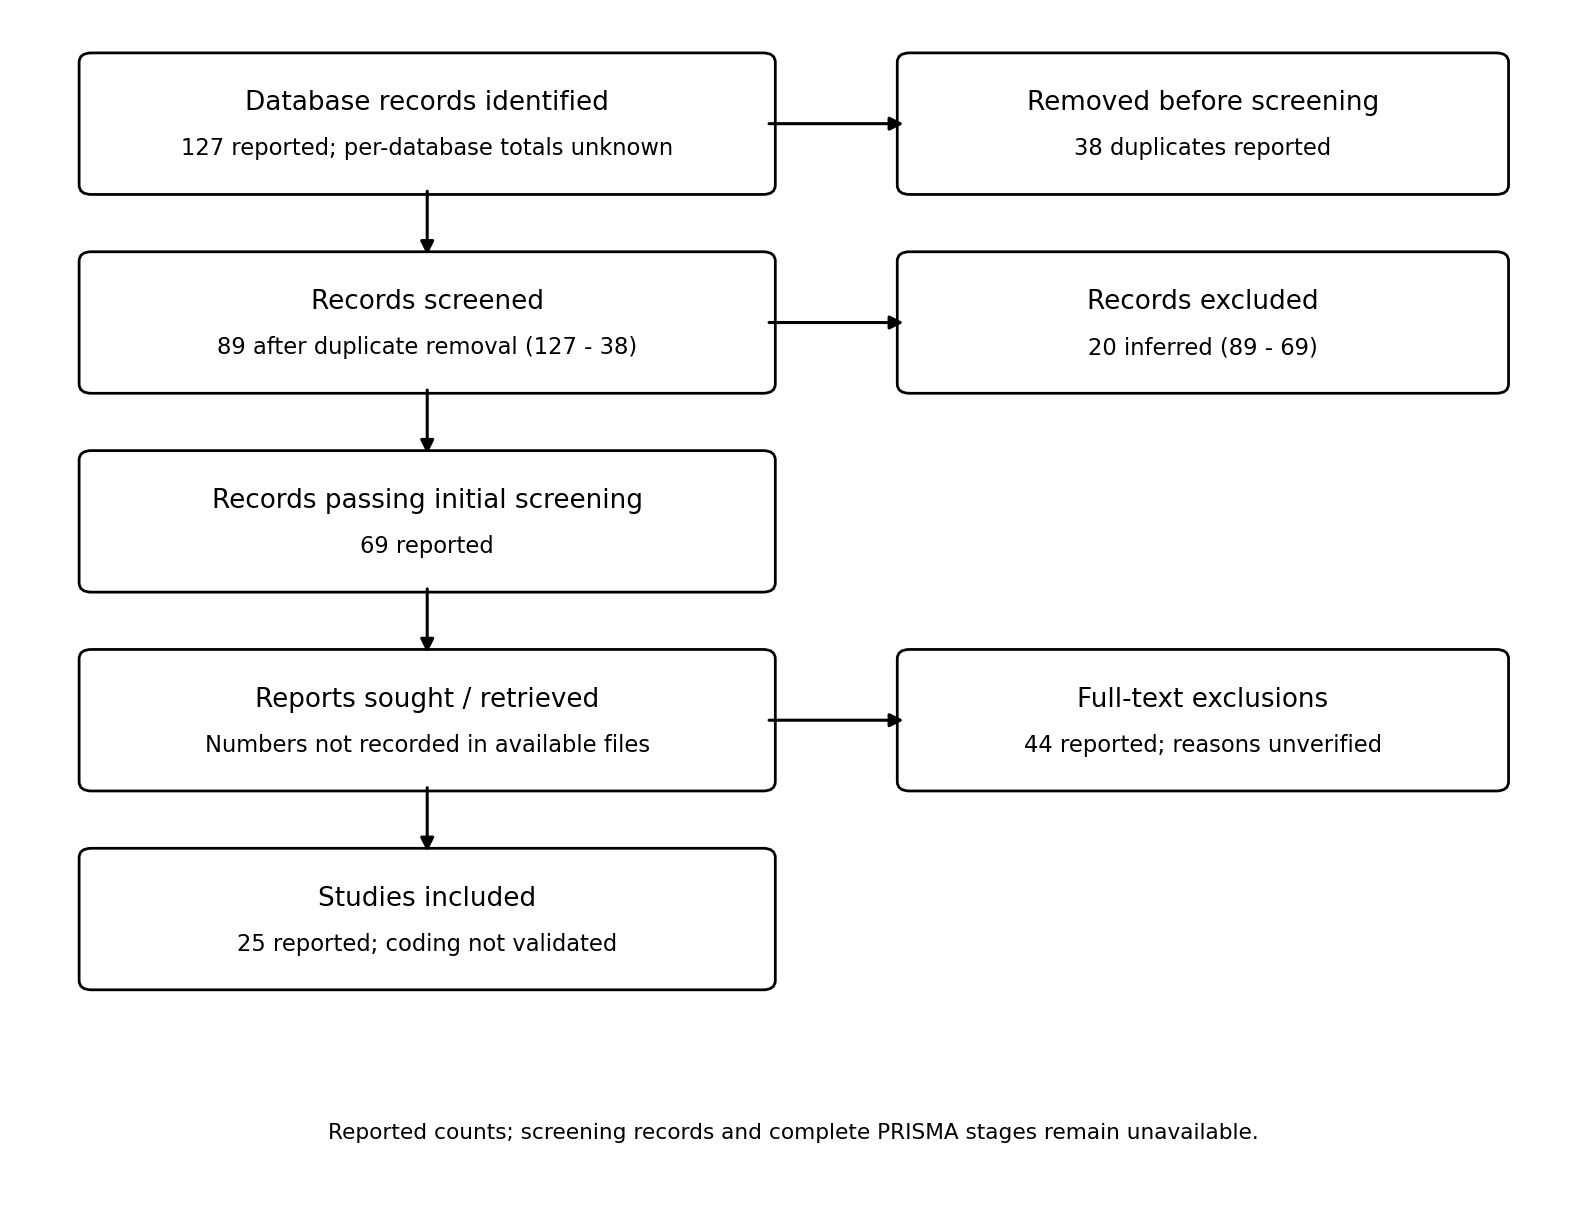
\includegraphics[width=0.90\textwidth]{figures/reported_prisma_flow.png}
\caption{Reported screening flow: 127 records and 25 retained publications. Counts are unverified against database exports or screening records; the flow is incomplete.}
\label{fig:prisma_reported}
\end{figure*}

Any repeated search should screen publication date and availability against a pre-declared window at the initial screening stage, document exceptions and preserve each exclusion decision. Whether the date window was applied to the reported screening cannot be verified. The bibliography lists years 2024--2026, but year alone does not establish availability at the reported August 2026 search date. A repeated search requires a new date and counts generated from its exports.

\subsection{Reference Inventory and Source Status}
\label{subsec:paperanalysis}

The bibliography lists 25 publications, described as 24 conference publications and one journal survey on the basis of the listed venues. This venue count is not a count of empirical implementations: reference~\cite{b15}, for example, is a conference review, while reference~\cite{b24} is a journal survey. Reference~\cite{b1} was described as conceptual. Full texts and the original coding file are needed to verify the classifications and identify the six publications excluded from the reported denominator of 19 implementations.

The companion \texttt{literature/papers.csv} and \texttt{literature/coding.csv} index all 25 bibliography entries and identify unassessed date, implementation and gap cells. As one limited example of a recoverable source observation, the IEEE abstract for~\cite{b3} describes a system ``powered by the ESP8266 micro controller''; this alone does not establish a measured physical-hardware evaluation. The source locator is in the companion evidence file. Short source extracts must be checked in context; absence claims require full-text inspection, not merely a silent abstract.

\subsection{Criteria for the Gap Analysis}
\label{subsec:gapsummary}

The seven positive criteria are: G1, one implementation combining encryption, access control, anomaly detection and compliance monitoring; G2, demonstrated local operation through connectivity loss; G3, continuous fusion of configuration, vulnerability and runtime information; G4, evaluation on constrained physical hardware; G5, use of deep learning or a transformer; G6, reporting the 95th percentile (P95) or P99 on the relevant path; and G7, closed-loop response from detection. G5 alone does not establish that a device's resource budget is exceeded. G2 does not by itself establish data sovereignty. Criteria and evidence locations must be checked consistently across included studies.

Table~\ref{tab:gapcounts} is generated from the evidence matrix. Only date-eligible, implemented systems with a source-supported coding decision contribute to each yes/coded count. Pending entries remain visible; the reported denominator of 19 implementations and its six exclusions are not reproducible from the available materials. Reference~\cite{b1} is not included in an implementation denominator merely because it appears in the bibliography. A defensible novelty statement requires completion of this review and comparison with current tools.

\begin{table}[t]
\caption{Evidence-coded counts for seven gap criteria}
\label{tab:gapcounts}
\centering\footnotesize\setlength{\tabcolsep}{3pt}
\begin{tabular}{@{}p{0.48\columnwidth}cc@{}}\toprule
\textbf{Criterion} & \textbf{Yes/coded} & \textbf{Pending}$^\dagger$ \\ \midrule
G1 Integrated controls & \textemdash & 25 \\
G2 Offline operation & \textemdash & 25 \\
G3 Dynamic fusion & \textemdash & 25 \\
G4 Constrained hardware & \textemdash & 25 \\
G5 Deep learning / transformer & \textemdash & 25 \\
G6 P95 or P99 reported & \textemdash & 25 \\
G7 Closed-loop remediation & \textemdash & 25 \\
\bottomrule\end{tabular}
\par\smallskip\parbox{\columnwidth}{\scriptsize $^\dagger$ Papers with unassessed date or implementation status, plus eligible implementations with this criterion unassessed. Yes/coded refers only to evidence-coded eligible implementations; it is not a complete-corpus rate while any are pending. A dash indicates no coded denominator.}
\end{table}


\section{Empirical Methodology and Rust Tooling Stack}
\label{sec:methodology}

This section sets out the hypotheses, proposed test conditions and available component measurements.

\subsection{Hypotheses and Decision Rules}
\label{subsec:hypothesis}

The following hypotheses specify a \emph{prospective} Ubuntu laptop-VM study. A synthetic detector has been executed in a K3s pod and a separate loopback pilot has been run. The full Kubernetes admission-to-log path, disconnected, degraded, intermittent or limited-bandwidth (DDIL) network, partition and comparator conditions remain untested.

\noindent\textbf{H1a --- detection, including DDIL (RQ1/RQ3/RQ4).} For every fixed event class in the baseline, independent-loss and burst-loss cells D0--D2, the two-sided 95\% Clopper--Pearson confidence interval (CI) for the event-level true-positive rate (TPR) has a lower bound of at least 90\%. Each cell requires at least 100 labelled events across 30 seeds, a fixed one-to-one matching window, and disclosure of false alerts per node-day. Event-level exact intervals assume independent Bernoulli outcomes; a seed-block bootstrap is reported as a clustering sensitivity, not proof of independence. The event classes, timing and matching window must be fixed before the future run. The supplied synthetic CPU-spike study alone cannot establish H1a.

\noindent\textbf{H1b --- latency (RQ2/RQ5).} On the target K3s VM, the seed-bootstrap 95\% upper bound for P99 scheduled-request-to-AdmissionReview-response latency, including the SQLite commit, is below 50~ms at each of 1, 10 and 100~requests/s for 1--50~KiB objects. The short-burst VM loopback pilot tests a narrower path and did not use the Kubernetes API.

\noindent\textbf{H1c --- CPU (RQ2/RQ5).} During a 24-hour VM trial, the agent's CPU time divided by elapsed time is below 10\% of one core. Measure its cgroup separately from K3s and background load.

\noindent\textbf{H1d --- memory (RQ2/RQ5).} During a 24-hour VM trial, the maximum sampled agent-cgroup \texttt{memory.current} is below 200,000,000 bytes. Report the sampling interval and K3s separately; sampled cgroup memory is not process resident set size (RSS) and may miss transient peaks.

\noindent\textbf{H1e --- comparator equivalence (RQ3).} For each predeclared event class and D0--D2 cell, let $\Delta$ be the TPR of LDPAD on K3s minus the TPR of the same detector on CRANE Cloud, in percentage points, using identical labelled event sets and matched seed runs. Paired two-one-sided testing (TOST) evaluates $-5< E[\Delta] <5$ at one-sided $\alpha=0.05$~\cite{b_tost}. Both one-sided tests must reject. An unadjusted 90\% paired-$t$ confidence interval should lie wholly within $(-5,+5)$; additionally, Holm-adjust the TOST $p$-values across the complete prespecified cell family and require each adjusted $p<0.05$. An interval inside the unadjusted bounds alone is insufficient after Holm correction. This is an equivalence margin of five \emph{percentage points}, not 5\% relative difference. Inference assumes independent seed-level pairs and an adequate paired-$t$ approximation. An inconclusive test establishes neither equivalence nor non-equivalence. No matched CRANE data exist here.

\noindent\textbf{H1f --- partition integrity (RQ4).} During a five-minute complete interruption of the remote link, the event-level TPR lower bound remains at least 90\% for each locally observable labelled event class; after reconnection, all expected local event records, checked against an independent label ledger, are delivered authenticated, without missing or duplicate entries, and in per-source sequence order within a predeclared observation window. The local application programming interface (API) and durable log remain available. The bounded trial does not prove correctness for every outage. This test is not yet run.

A claimed overall result requires the relevant thresholds and comparisons to be met in the planned cells. Results may also be inconclusive; failure to establish a target is not automatically evidence that its opposite is true. Detection, latency, resource use, equivalence and partition integrity are reported separately.

\subsection{Independent and Dependent Variables}
\label{subsec:variables}

{Independent variables:} planned DDIL condition D0--D3 (Section~\ref{subsec:chaos}); admission request rate (1, 10, 100/s); and labelled event class. Bandwidth and routing must be fixed and recorded for the comparison. The detector's VM test used one K3s node; any 3-, 5- or 8-node scenarios are separate future simulations. The loopback latency pilot did not use K3s.

{Dependent variables:} P99 policy-decision latency; TPR for labelled events; clean-tick false-alert rate and operational alerts per node-day; CPU utilisation \%; random-access memory (RAM) in MB; recovery time after fault; data-loss window.

{Controlled variables:} Earlier detector components used a shared AMD EPYC~9V74 host. The latency pilot used an Ubuntu laptop VM on an Intel Core i5-7300U; the guest reported an ext2/ext3 filesystem type and unspecified backing media. Before the later K3s test, a VM snapshot reported 5.7~GiB total and 3.9~GiB available memory; this is not an agent resource measurement. The guest CPU allocation, hypervisor version, storage hardware, power and thermal conditions were not captured. The seeded detector used the documented synthetic trace and a 30-tick warm-up. The latency pilot used the object-size mix in Section~\ref{subsec:latency_pilot}; no explicit CPU pinning or latency warm-up was recorded.

\subsection{Experimental Design Discipline}
\label{subsec:design}

The prospective comparison uses 30 matched seeds, interleaved arm order and identical labelled event lists. The seed list and fixed parameters of the exploratory Rust generator are included in the companion package. The original command-line interface (CLI) used \texttt{thread\_rng} and did not save generator seeds; its captured outcomes can be reanalysed but not recreated as identical new runs. The separate seeded Rust component used seeds 0--29, and the fixed MadSim scenarios used seed 0; these are not the future VM comparisons.

The prospective analysis-plan commit is \texttt{7ece8}\allowbreak\texttt{d053e}\allowbreak\texttt{73edf}\allowbreak\texttt{46656}\allowbreak\texttt{83d72}\allowbreak\texttt{a7d94}\allowbreak\texttt{83dc8}\allowbreak\texttt{bfcc1}, dated 1 November 2026, 21:35:58 UTC+03:00. The bundled local Git object records this working plan before the still-unrun VM/DDIL/CRANE comparison, but is not independently timestamped registration; an author-reviewed addendum must fix the event classes, matching window, family and observation durations before data collection. Earlier x86 and simulation explorations preceded this plan and are not pre-registered by it. The separate fusion-design commit is \texttt{e4cbc}\allowbreak\texttt{35665}\allowbreak\texttt{b51cc}\allowbreak\texttt{1fbe0}\allowbreak\texttt{bb137}\allowbreak\texttt{52c81}\allowbreak\texttt{41b4e}\allowbreak\texttt{e560a}, dated 1 November 2026, 20:23:31 UTC+03:00; it records synthetic scenario design only and does not register the comparator study.

\subsection{Core Rust Toolchain}
\label{subsec:rusttoolchain}

Table~\ref{tab:rusttoolchain} is generated from the Rust manifests and records direct dependencies and prototype status.

\begin{table}[ht]
\caption{Rust Crates Used in the Current LDPAD Harness}
\label{tab:rusttoolchain}
\centering
\setlength{\tabcolsep}{2pt}
\begin{tabular}{|p{55pt}|p{85pt}|p{60pt}|}
\hline
\textbf{Layer} & \textbf{Crate} & \textbf{Status} \\
\hline
Serialisation & \texttt{serde}, \texttt{serde\_json} & In use \\
Hashing & \texttt{sha2}, \texttt{hex} & In use \\
Randomness & \texttt{rand}, \texttt{rand\_distr} & In use \\
CLI & \texttt{clap} & In use \\
Tail latency & \texttt{hdrhistogram} & Pilot \\
Benchmarking & \texttt{criterion} & Dev dependency \\
Async runtime & \texttt{tokio} & Latency pilot \\
Policy and log & \texttt{regorus}, \texttt{rusqlite} & Latency pilot \\
Statistics & in-house \texttt{stats.rs} & In use \\
Deterministic simulation & \texttt{madsim} & Separate prototype \\
Other planned services & \texttt{turmoil}, \texttt{openraft}, \texttt{tonic} & Not direct dependencies \\
\hline
\end{tabular}

\end{table}

\subsection{Standalone Rust Harness Results}
\label{subsec:measured}

The supplied Rust project was built with its locked dependencies on Ubuntu~24.04.3, Linux x86\_64, on an AMD EPYC~9V74 host using Rust~1.99.1. All fourteen defined tests passed in that earlier host run. The later VM test record and K3s-pod execution are reported separately in Section~\ref{sec:production}.

The original CLI was executed 30 times with 500 samples and a CPU spike scheduled every 50 samples (ten scheduled spikes per run). It uses \texttt{thread\_rng} without recorded seeds. Across these runs, the CLI printed a mean of 17.67 anomaly-alert ticks per run (95\% percentile bootstrap interval 16.73--18.60), with a range of 12--24. Every run reported 500 Normal ticks and peak risk 45.00. The captured run-level median is 18 alerts (first and third quartiles (Q1--Q3) 16--19.75; interquartile range (IQR) 3.75; 95\% bootstrap interval for the median 16.5--18.5). As the unmodified CLI reports only aggregate alerts, these counts alone do not establish true- or false-positive rates. Table~\ref{tab:ci} summarises this run; a separately instrumented seeded detector experiment is reported in Section~\ref{subsec:rust_seeded}.

\begin{table}[ht]
\caption{Unseeded Rust CLI on x86\_64: 30 runs of 500 ticks each}
\label{tab:ci}
\centering
\footnotesize
\setlength{\tabcolsep}{3pt}
\begin{tabular}{@{}lr@{}}
\toprule
\textbf{Measure} & \textbf{Observed} \\
\midrule
CLI repetitions & 30 \\
Samples / scheduled spikes per run & 500 / 10 \\
Alert ticks/run, mean (95\% CI) & 17.67 (16.73--18.60) \\
Alert ticks/run, median (Q1--Q3) & 18 (16--19.75) \\
IQR (Q3--Q1) & 3.75 \\
Median, 95\% bootstrap CI & 16.5--18.5 \\
Alert ticks/run, range & 12--24 \\
Normal ticks/run & 500 \\
\bottomrule
\end{tabular}

\end{table}

A separate 100,000-observation component run of the anomaly detector printed the median (P50), P95, and P99 as 0~µs. The code truncates elapsed times to integer microseconds, so these printed zeros do not mean zero latency; the tail is unresolved at this precision. This is not end-to-end policy-to-durable-log latency and cannot establish the VM latency hypothesis.


\subsection{Laptop-VM Loopback Policy and SQLite Latency Pilot}
\label{subsec:latency_pilot}

A new exploratory Rust harness sends synthetic AdmissionReview JavaScript Object Notation (JSON) over localhost Hypertext Transfer Protocol (HTTP) to a server that evaluates one real Regorus 0.14 policy and writes the decision and object digest to SQLite 3.50.2. The response is sent after the transaction commits in write-ahead logging (WAL) mode with \texttt{synchronous=FULL}~\cite{b_latency_sqlite}. This harness is separate from the supplied detector and does not run the Kubernetes API, K3s, or the proposed production service. A successful commit and storage-sync call do not by themselves demonstrate survival of power loss on an arbitrary device.

A Tokio generator schedules requests without waiting for preceding responses. Each of 30 seeds shuffles the order of the 1, 10 and 100~request/s conditions; each condition contains ten requests, two each with object sizes of 1, 4, 10, 25 and 50~KiB. The 100~request/s condition is therefore a set of short bursts rather than sustained load. All 900 completed requests matched their unique identifier (UID) and decision in the SQLite log. The pilot ran on an Ubuntu x86\_64 laptop VM with an Intel Core i5-7300U; the guest reported an ext2/ext3 filesystem type, and the physical backing media were not recorded.

The primary latency runs from scheduled arrival to the complete HTTP response after commit; it includes generator scheduling delay and loopback transport. Raw observations use nanosecond units, and Table~\ref{tab:latency_pilot} reports their nearest-rank percentiles. A separate high-dynamic-range (HDR) \texttt{hdrhistogram} uses \texttt{record\_correct} at the intended interval as a sensitivity analysis~\cite{b_latency_hdr}; unexpanded open-loop observations are primary. At 100~requests/s the corrected HDR contained 303 rather than 300 samples, with P99 17.220~ms versus 15.884~ms in the uncorrected HDR. The latter differs slightly from the 15.881~ms raw nearest-rank estimate because of histogram quantisation. A Linux probe measured \texttt{fsync}/\texttt{fdatasync} calls during each commit. Sync share is their summed duration divided by summed server accept-to-commit time, not total experiment wall time.

\begin{table*}[t]
\caption{Laptop-VM loopback latency pilot: 30 seeds, 300 requests per rate, and 95\% seed-bootstrap intervals}
\label{tab:latency_pilot}
\centering
\small
\textbf{Observed values}\par\smallskip
% BEGIN GENERATED LATENCY POINT TABLE
\begin{tabular}{@{}rrrrrrr@{}}
\toprule
\textbf{Rate} & \textbf{P50} & \textbf{P95} & \textbf{P99} & \textbf{P99.9} & \textbf{Max} & \textbf{Sync} \\
\textbf{req/s} & \textbf{ms} & \textbf{ms} & \textbf{ms} & \textbf{ms} & \textbf{ms} & \textbf{\%} \\
\midrule
1 & 5.827 & 12.266 & 13.342 & 48.029 & 48.029 & 91.2 \\
10 & 4.698 & 7.652 & 29.812 & 143.758 & 143.758 & 86.0 \\
100 & 3.266 & 5.522 & 15.881 & 33.989 & 33.989 & 72.7 \\
\bottomrule
\end{tabular}

% END GENERATED LATENCY POINT TABLE

\medskip
\textbf{95\% intervals from 10,000 resamples of seed blocks}\par\smallskip
% BEGIN GENERATED LATENCY CI TABLE
\begin{tabular}{@{}rrrrrr@{}}
\toprule
\textbf{Rate} & \textbf{P50} & \textbf{P95} & \textbf{P99} & \textbf{P99.9} & \textbf{Sync} \\
\textbf{req/s} & \textbf{ms} & \textbf{ms} & \textbf{ms} & \textbf{ms} & \textbf{\%} \\
\midrule
1 & [4.948, 10.154] & [11.839, 12.408] & [12.889, 14.737] & [13.342, 48.029] & [89.8, 92.3] \\
10 & [3.859, 5.044] & [6.472, 14.082] & [8.372, 56.075] & [16.117, 143.758] & [81.2, 90.3] \\
100 & [3.119, 3.400] & [4.489, 11.682] & [5.265, 25.415] & [7.211, 33.989] & [71.2, 74.4] \\
\bottomrule
\end{tabular}

% END GENERATED LATENCY CI TABLE
\end{table*}

Each rate has 300 observations, so nearest-rank P99.9 equals the maximum; its bootstrap interval cannot estimate unseen extremes. At 10~requests/s, the P99 upper bound was 56.075~ms and the maximum was 143.758~ms. Thus, the pilot did not meet the 50~ms upper-bound rule at every rate. These short-burst intervals are exploratory and do not capture all host, time and hardware variation; this loopback pilot does not establish H1b for the deployed K3s path.

\subsection{Fault, Network, and Chaos Emulation}
\label{subsec:chaos}

The planned dedicated-test-interface conditions are D0: no imposed impairment; D1: 300~ms one-way egress delay with 20\% independent loss; D2: 300~ms one-way delay and Gilbert--Elliott burst loss; and D3: a five-minute complete remote-link partition for H1f. For D2, the proposed \texttt{netem} transition parameters are $p=2.5\%$, $r=10\%$, bad-state loss 100\%, and good-state loss 0\%, giving 20\% ideal stationary loss. The realised loss, delay, both directions, packet counters, seed, interface and routing must be recorded; TCP retransmissions and finite samples affect observed behaviour. Labels must traverse the impaired path for H1a. D3 must not disconnect the local API or log. The commands and limitations are included as a plan only~\cite{b_netem}; no DDIL condition was run.

\subsection{Statistical Checklist}
\label{subsec:stats}

For each seed/run, report the median, Q1, Q3 and IQR and a 95\% percentile bootstrap interval with 10,000 resamples of independent run units; matched comparisons resample whole seed pairs. The current unseeded capture uses a run-level bootstrap, while the seeded detector uses seed-level blocks. For \emph{independent} groups, the prospective analysis reports a two-sided, tie-corrected Mann--Whitney U and Cliff's $\delta=P(X>Y)-P(X<Y)$. For \emph{paired} seed runs, it reports the paired difference and Hedges $g_z$, the small-sample-corrected mean paired difference divided by the standard deviation of paired differences. This effect size does not replace TOST. The prospective H1e family uses Holm-adjusted TOST $p$-values. Statistical functions have been checked against SciPy to an absolute tolerance of $10^{-9}$ where a corresponding SciPy reference is available; Holm was checked against known values. None of these comparison statistics is reported as an experimental result without matched comparator observations.

\section{Proposed LDPAD Framework}
\label{sec:ldpad}

This section presents the proposed architecture. Unless explicitly identified as implemented or measured, the controls and interactions below are design requirements rather than deployed capabilities.

\subsection{Design Goals, Non-Goals, and the Constraint Envelope}
\label{subsec:goals}

LDPAD is specified around measurable design goals for an environment where a wide-area network (WAN) link may be unavailable. Table~\ref{tab:goals} lists targets and proposed assessment methods; several require components or trials not yet available. The 72-hour offline target requires a longer trial than the five-minute partition proposed for H1f.

\begin{table}[ht]
\caption{Proposed LDPAD Design Goals and Assessment Methods}
\label{tab:goals}
\centering
\setlength{\tabcolsep}{3pt}
\begin{tabular}{|>{\raggedright\arraybackslash}p{58pt}|>{\raggedright\arraybackslash}p{62pt}|>{\raggedright\arraybackslash}p{58pt}|}
\hline
\textbf{Goal} & \textbf{Quantitative target} & \textbf{Planned check} \\
\hline
Detection fidelity & Per-cell 95\% exact TPR lower bound $\geq$90\%; clean-tick alert rate $\leq$5\% & Labelled-event and clean-trace analysis \\
\hline
Decision latency & 95\% P99 upper bound $<$50~ms & Instrumented request path \\
\hline
CPU overhead & $<$10\% of one core over 24~h & cgroup v2 \texttt{cpu.stat} \\
\hline
Memory overhead & $<$200~MB agent cgroup & cgroup v2 \texttt{memory.}\allowbreak\texttt{current} \\
\hline
Offline autonomy & $\geq$72~h full function, no WAN & 72-h partition trial \\
\hline
Determinism & Byte-identical results for a fixed seed & \texttt{madsim} replay \\
\hline
Auditability & Every state change hash-chained & Oplog verifier \\
\hline
\end{tabular}
\end{table}

\noindent\textbf{Explicit non-goals.} LDPAD is not a SIEM replacement, zero-day detector, multi-cluster control plane or certification instrument. The planned single-node agent should monitor without continuous supervision; high-impact actions require operator confirmation or the multi-node quorum gate described in Layer~8.

\noindent\textbf{VM evaluation profile.} Table~\ref{tab:envelope} distinguishes the observed guest memory from proposed allocations and framework targets. The K3s server minimum is documented as two cores and 2~GB of RAM~\cite{b_k3s_requirements}. The VM snapshot reported 5.7~GiB total memory; its CPU allocation, hypervisor version and backing storage have not been independently recorded. A virtual resource limit does not reproduce the CPU architecture, storage, power or thermal behaviour of a dedicated edge device.

\begin{table}[ht]
\caption{Laptop-VM Profile and Proposed Framework Targets}
\label{tab:envelope}
\centering
\setlength{\tabcolsep}{3pt}
\begin{tabular}{|>{\raggedright\arraybackslash}p{42pt}|>{\raggedright\arraybackslash}p{66pt}|>{\raggedright\arraybackslash}p{66pt}|}
\hline
\textbf{Resource} & \textbf{VM profile} & \textbf{LDPAD target} \\
\hline
RAM & 5.7~GiB guest (observed) & $<$200~MB agent cgroup \\
CPU & 2 vCPUs (proposed) & $<$10\% of one core \\
Storage & Laptop-backed guest disk & $\leq$50~MB oplog + 256~MB images \\
Network & DDIL (planned) & Degrade, never block \\
Power & Host AC/battery & Record power mode \\
Thermal & Host-dependent & Record throttling \\
\hline
\end{tabular}
\end{table}

\subsection{Architectural Principles and What They Rule Out}
\label{subsec:principles}

The LDPAD design follows six principles, each stated with the design option it forecloses.

\begin{enumerate}
\item \textbf{Simplicity over sophistication.} Prefer the simplest mechanism that meets the target. \emph{Rules out:} deep learning, reinforcement learning, and transformer-based detection in the critical path.
\item \textbf{Offline-first.} Every layer must produce a correct (possibly degraded) answer with the WAN down. \emph{Rules out:} cloud-hosted policy engines, remote key servers, and any synchronous network call on the decision path.
\item \textbf{Resource-aware.} Security intensity scales with available headroom. \emph{Rules out:} fixed-cadence full-cluster scans and unbounded telemetry buffers.
\item \textbf{Dynamic posture.} Posture is a continuous function of configuration, threat, and runtime state, not a deployment-time verdict. \emph{Rules out:} one-shot cloud security posture management (CSPM) scans and static admission-only enforcement.
\item \textbf{Incremental deployability.} Each layer should be independently useful and independently removable. \emph{Rules out:} monolithic agents and all-or-nothing rollout.
\item \textbf{Minimal dependency surface.} The supplied manifest lists twelve direct runtime dependencies, with versions resolved in \texttt{Cargo.lock}; the supplied archive does not vendor their source. Reducing additional deployment dependencies is a design goal.
\end{enumerate}

\subsection{Reference Architecture, Layer Map, and Trust Boundaries}
\label{subsec:ldpad_arch}

The proposed baseline draws on Center for Internet Security (CIS) guidance and the proposed anomaly monitor uses an exponentially weighted moving average (EWMA); the supplied detector instead uses a rolling window. Threat information includes Common Vulnerabilities and Exposures (CVE) identifiers. Figure~\ref{fig:ldpad_flow} and Table~\ref{tab:ldpadlayers} show the intended control flow and responsibilities. JSON Web Tokens (JWT), Transport Layer Security (TLS), mutual TLS (mTLS), keyed-hash message authentication codes (HMAC), time-to-live (TTL) and out-of-memory (OOM) are used in the design. Resource figures are targets, not measurements; offline operation and reconnection remain unverified.

\begin{figure}[t]
\centering
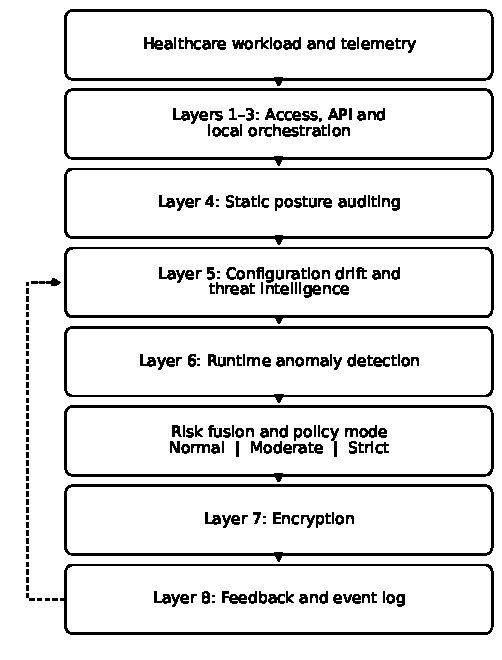
\includegraphics[width=\columnwidth]{figures/architecture_single_column.pdf}
\caption{Proposed LDPAD control flow through Layers~1--8. The unified risk score combines static, drift, threat and anomaly signals and selects Normal, Moderate or Strict mode. The dashed arrow denotes feedback.}
\label{fig:ldpad_flow}
\end{figure}

\begin{table*}[t]
\caption{Proposed 8-Layer LDPAD Architecture for Resource-Constrained Healthcare Workloads}
\label{tab:ldpadlayers}
\centering
\setlength{\tabcolsep}{4pt}
\begin{tabular}{|c|p{64pt}|p{118pt}|p{94pt}|p{62pt}|}
\hline
\textbf{Layer} & \textbf{Name} & \textbf{Core Mechanism} & \textbf{Proposed Target} & \textbf{Failure Mode} \\
\hline
1 & User / Application & Clinical portals, telemedicine clients, IoMT dashboards; thin browser or native client & Runs on clinician device & Client-side credential theft \\
\hline
2 & API \& Service & gRPC/Protobuf service interfaces; JWT bearer auth; mTLS between services & $<$10~MB RSS & Token replay; clock skew \\
\hline
3 & Lightweight Orchestration & K3s single binary with SQLite datastore; cgroup~v2; local state cache in WAL mode for offline operation & $\leq$150~MB RSS baseline & OOM kill; kubelet restart loop \\
\hline
4 & Static Posture Auditing & Seven proposed Rego rules; separate simplified Rust predicates are tested & $<$5~ms eval; 20~MB RSS & Policy timeout; malformed object \\
\hline
5 & Dynamic Posture Management & Drift detector $+$ threat-intel matcher $+$ risk fusion $+$ hysteretic policy adapter $+$ temporal tracker & $<$5\% CPU; 30~s cadence & Stale risk score; intel TTL expiry \\
\hline
6 & Runtime Anomaly Detection & EWMA-based 3-sigma monitor over five metrics, with persistence and cooldown & $<$3\% CPU; $\sim$1~MB RSS & False-positive spike; cold-start blindness \\
\hline
7 & Lightweight Encryption & AES-256-GCM field encryption; SHA-256 HMAC integrity; envelope key hierarchy; TLS~1.3 via rustls & $<$2\% CPU & Key corruption; nonce reuse \\
\hline
8 & Evaluation \& Feedback Loop & Threshold response, manual override, posture update; closed-loop remediation ladder and offline reconciliation on reconnect & Action $\leq$200~ms (rungs 1--4) & Cascading quarantine \\
\hline
\end{tabular}
\end{table*}

\noindent\textbf{Trust boundaries.} Table~\ref{tab:trust} lists four proposed boundaries and controls. A complete end-to-end flow can cross several boundaries in sequence.

\begin{table}[ht]
\caption{Proposed Trust Boundaries and Their Controls}
\label{tab:trust}
\centering
\setlength{\tabcolsep}{3pt}
\begin{tabular}{|p{40pt}|p{52pt}|p{62pt}|}
\hline
\textbf{Boundary} & \textbf{Separation} & \textbf{Control} \\
\hline
TB1 & Workload $\rightarrow$ LDPAD agent & Unix domain socket; peer-cred check \\
\hline
TB2 & Agent $\rightarrow$ Kernel/API & Scoped ServiceAccount; no cluster-admin \\
\hline
TB3 & Node $\rightarrow$ WAN & rustls TLS 1.3; pinned certificate authority (CA); no inbound \\
\hline
TB4 & Operator $\rightarrow$ Agent & mTLS client cert; 2-of-3 quorum for rungs 5--7 \\
\hline
\end{tabular}
\end{table}

\noindent\textbf{Deployment topology.} The proposed topology uses an \texttt{ldpad-}\allowbreak\texttt{node} agent per node in a DaemonSet and an \texttt{ldpad-}\allowbreak\texttt{posture} controller in a Deployment. The agent would own Layers~3, 4, 6, 7 and part of~8; the controller would own Layer~5 and cluster-scoped actions. Each node would keep a local SQLite database. Cluster risk is proposed to use a weighted maximum of node scores; its resistance to falsified node inputs is untested.

\subsection{Proposed End-to-End Control Loop}
\label{subsec:loop}

The proposed LDPAD control loop has five stages and two cadences. The \emph{fast path} (Layer~6) would run per telemetry sample; the \emph{slow path} (Layers~4--5) would run every 30~s and on Kubernetes watch events.

\begin{table}[ht]
\caption{Proposed Control Loop Stages and Cadence}
\label{tab:loop}
\centering
\setlength{\tabcolsep}{3pt}
\begin{tabular}{|c|p{42pt}|p{52pt}|p{38pt}|}
\hline
\textbf{Stage} & \textbf{Action} & \textbf{Input} & \textbf{Cadence} \\
\hline
S1 Observe & Sample 5 metrics; hash watched resources & cgroup, kube watch & 1~s (fast) \\
\hline
S2 Evaluate & Score drift, threat, anomaly & Baselines, CVE bundle & 30~s / event \\
\hline
S3 Fuse & Compute unified RiskScore & Four risk components & 30~s \\
\hline
S4 Decide & Select mode with hysteresis & RiskScore, trend slope & 30~s \\
\hline
S5 Act & Emit finding, apply remediation rung & Mode, finding class & On change \\
\hline
\end{tabular}
\end{table}

The design requires stage outputs to reach the Layer~8 oplog before downstream use. The supplied prototype does not implement this complete loop or establish crash-replay guarantees.

\subsection{Layer 1 --- User / Application}
\label{subsec:layer1}

Layer~1 represents proposed clinical-facing clients, such as browser portals, mobile telemedicine applications and IoMT dashboards. The design does not instrument clients; it proposes short-lived bearer tokens, origin-bound sessions and authentication at Layer~2. Client compromise remains an assumed threat. These controls have not been evaluated in a clinical deployment.

\subsection{Layer 2 --- API \& Service}
\label{subsec:layer2}

Layer~2 is the proposed service interface between clinical clients and registry workloads. It specifies gRPC/Protobuf, locally verified JWTs, mutual TLS and request-shape validation. The under-10~MB RSS figure is an unmeasured target; comparative wire cost and the full service path have not been tested.

\subsection{Layer 3 --- Lightweight Orchestration}
\label{subsec:layer3}

Layer~3 provides the orchestration substrate. On an Ubuntu VM, K3s hosted the test pod in which the Rust prototype and seeded detector were executed; this demonstrates execution in K3s. The design additionally proposes continuous local metric collection, a SQLite state cache and restricted agent privileges. The supplied CLI does not implement the local cache and reconciliation path needed for the proposed H1f partition test. Relative memory use across Kubernetes distributions remains unmeasured.

\subsection{Layer 4 --- Static Posture Auditing}
\label{subsec:layer4}

The supplied Rust component audits fields of a simplified Kubernetes-style resource using seven predicate functions. Table~\ref{tab:rules} is generated from those functions and their weights. The proposed full AdmissionReview/Rego integration and associated resource budget are not established by this component; the separate loopback latency pilot evaluates a different Regorus policy.

\begin{table}[ht]
\caption{The Seven Rules in the Supplied Rust Auditor}
\label{tab:rules}
\centering
\setlength{\tabcolsep}{3pt}
\begin{tabular}{|c|p{0.60\columnwidth}|r|}
\hline
\textbf{ID} & \textbf{Rust auditor rule} & \textbf{Weight} \\
\hline
R1 & \texttt{non\_privileged} & 30 \\
\hline
R2 & \texttt{non\_root} & 20 \\
\hline
R3 & \texttt{read\_only\_rootfs} & 15 \\
\hline
R4 & \texttt{network\_policy\_present} & 20 \\
\hline
R5 & \texttt{rbac\_least\_privilege} & 15 \\
\hline
R6 & \texttt{image\_not\_latest} & 10 \\
\hline
R7 & \texttt{resource\_limits\_set} & 10 \\
\hline
\end{tabular}

\end{table}

\noindent\textbf{Evaluation and failure policy.} A future policy adapter would evaluate admission objects and apply the proposed mode-specific timeout policy; that integration remains untested. For the supplied auditor, the static score is a severity-weighted failure ratio:
\begin{equation}
r_s = \frac{\sum_{i \in F} w_i}{\sum_{i=1}^{7} w_i}
\label{eq:static}
\end{equation}
where $F$ is the set of failing rules for one resource. The seven source-code weights total 120 per resource. The supplied auditor reports $100r_s$; for multiple resources it sums failed and total weights across resources before multiplying by 100.

\subsection{Layer 5 --- Dynamic Posture Management}
\label{subsec:layer5}

Layer~5 is the paper's proposed dynamic-posture contribution; its novelty requires the outstanding literature review. The design specifies five cooperating components within a \texttt{tokio} task and a bounded channel to Layer~8. The evaluated CLI combines simplified static, drift and anomaly scores, but does not implement the complete proposed pipeline for continuous posture assessment.

\subsubsection{Component 5.1 --- Configuration Drift Detector}
\label{subsubsec:drift}

\noindent\textbf{Baseline construction.} The proposed detector canonicalises each watched object, hashes it with SHA-256 and stores signed Merkle roots. An individual resource proof would cost $O(\log n)$ hashes. The supplied Rust detector instead hashes the provided JSON string and returns a changed-current-resource fraction; it does not implement canonicalisation, Merkle proofs or detection of removed objects.

\noindent\textbf{Scan strategy.} The design proposes full reconciliation every 30~s and incremental re-hashing driven by Kubernetes watch events. The watch path is what makes drift detection \emph{continuous} rather than periodic, and is a proposed design choice, not a measured distinction from every CSPM tool.

\noindent\textbf{Drift classification.} Each divergence is assigned a class and severity: \textsc{Removed} (0.9) $>$ \textsc{Added} (0.6) $>$ \textsc{Modified} (0.3). Severity is multiplied by a namespace criticality tier $c_d \in \{0.5, 1.0, 1.5\}$ (low, clinical, identity/key material). The contribution saturates so that a hostile actor cannot drive the score to infinity by mass-creating resources:
\begin{equation}
\text{DriftRisk} = \min\!\left(1,\;
\frac{\sum_{d} s_d \cdot c_d}{D_{\max}}\right), \quad D_{\max} = 5.
\label{eq:drift}
\end{equation}

\begin{figure}[ht]
\caption{Proposed Configuration Drift Detection (per 30~s cycle, Layer 5)}
\label{alg:drift}
\begin{algorithmic}[1]
\STATE $W \leftarrow$ watch\_events\_since($t-30$)
\FORALL{$o \in W$}
    \STATE $j \leftarrow \textsc{JcsCanonicalise}(o.\text{spec})$
    \STATE $h \leftarrow \textsc{Sha256}(j)$
    \IF{$h \neq \text{baseline}[o.\text{key}]$}
        \STATE $c \leftarrow \textsc{Classify}(\text{baseline}, o)$
        \STATE \textbf{emit} $DriftRecord\{o.\text{key}, c, \dots\}$
    \ENDIF
\ENDFOR
\STATE $r \leftarrow \min(1,\ \sum s_d c_d / 5)$
\STATE \textbf{return} $r$
\end{algorithmic}
\end{figure}

\subsubsection{Component 5.2 --- Threat Intelligence Integrator}
\label{subsubsec:intel}

\noindent\textbf{Sources and offline operation.} The design proposes locally signed snapshots of National Vulnerability Database (NVD), CISA Known Exploited Vulnerabilities (KEV) and OSV data. A trusted operator would verify source provenance and sign each snapshot manifest; upstream Ed25519 signatures are not assumed. On expiry after 72 hours without WAN, the proposed adapter would raise \textsc{IntelStale} and impose a Moderate mode floor outside Eq.~\ref{eq:guarded_fusion}. The supplied store only matches strings and scores severity times likelihood; signed feeds and the stale-intelligence mode floor are not implemented.

\noindent\textbf{Matching.} The design proposes a CycloneDX software bill of materials (SBOM) generated per pod start and Common Platform Enumeration (CPE) matching against that SBOM. This proposed path does not require execution of untrusted code or a filesystem scan; it is not implemented in the supplied matcher.

\noindent\textbf{Scoring.} The proposed threat score uses the worst match, with a KEV boost and an exposure discount for services not reachable from the clinical virtual local area network (VLAN). CVSS denotes the Common Vulnerability Scoring System:
\begin{equation}
\begin{aligned}
\text{ThreatRisk} = \min\!\Bigl(1,\; &E\max_k\bigl[
\tfrac{\text{CVSS}_k}{10} \\
&{}\cdot(1 + 0.5\,\text{KEV}_k)\bigr]\Bigr).
\end{aligned}
\label{eq:threat}
\end{equation}
with $E \in \{0.3, 0.6, 1.0\}$ for isolated, internal-only, and externally-exposed services respectively.

\subsubsection{Component 5.3 --- Risk Fusion}
\label{subsubsec:fusion}

Let $r_s,r_d,r_t,r_a\in[0,1]$ denote the static, drift, threat and anomaly risks. The linear score on a 0--100 scale is
\begin{align}
S_L &= 100\bigl(\alpha r_s+\beta r_d \nonumber\\
&\quad{}+\gamma r_t+\delta r_a\bigr).
\label{eq:fusion}
\end{align}
Here $\alpha=0.30$, $\beta=0.25$, $\gamma=0.25$, and $\delta=0.20$. The supplied Rust scorer takes inputs on a 0--100 scale and implements the equivalent weighted sum. Its instantaneous mode is Strict for a score $>80$, Moderate for a score $>50$, and Normal otherwise; the supplied CLI has no hysteretic adapter. With only static risk 0.9, the linear score is 27.00; with only threat risk 0.9, it is 22.50. Both therefore yield Normal under the implemented thresholds.

\noindent\textbf{Guarded candidate.} A separate experimental Rust implementation evaluates
\begin{equation}
\begin{aligned}
S_G=\max\!\Bigl(&S_L,\;51\,\mathrm{1}_{\max(r_s,r_d,r_t)\geq0.90},\\
&81\,\mathrm{1}_{r_a\geq0.90}\Bigr).
\end{aligned}
\label{eq:guarded_fusion}
\end{equation}
The floors encode the desired response to high single-source risk; they are design choices, not independently validated severity labels. With three consecutive one-second runtime observations $r_a\geq0.90$, the candidate also permits a direct transition to Strict. The original CLI continues to use the linear scorer. Section~\ref{subsec:fusion_eval} evaluates the new component in simulation.

For comparison, a normalised weighted noisy-OR score is $S_O=100[1-\prod_i(1-w_i r_i)]/[1-\prod_i(1-w_i)]$, with non-negative weights summing to one. Normalisation makes the all-ones risk vector score 100. This is a scoring heuristic, not a calibrated probability of compromise.

\noindent\textbf{Worked example.} Consider a single resource with rules R1, R2 and R3 failing. Their weights are $30$, $20$ and $15$, so $r_s=65/120\approx0.5417$. One removed high-criticality object gives $\text{DriftRisk}=0.9\cdot1.5/5=0.270$. A KEV-listed CVE at CVSS~9.8 on an internally exposed service gives $\text{ThreatRisk}=0.98\cdot1.5\cdot0.6=0.882$. With two metrics persistently breaching at $z=4.2$, the proposed anomaly contribution is $\text{AnomalyRisk}=\min(1,4.2/6)=0.700$. Substitution into Eq.~\ref{eq:fusion} gives
\begin{align}
S_L &= 100\,(0.30\cdot\tfrac{65}{120}+0.25\cdot0.270 \nonumber\\
&\quad +0.25\cdot0.882+0.20\cdot0.700) \nonumber\\
&=100\,(0.5905)=59.05.
\end{align}
The linear thresholds therefore yield an instantaneous Moderate score. The proposed network restriction is not exercised by this calculation.

\noindent\textbf{Weight sensitivity.} Section~\ref{subsec:fusion_eval} reports a 0.05-step grid of 1,771 weight vectors against six synthetic design-labelled scenarios. It is not a sensitivity analysis of the 25 literature papers.

\subsubsection{Component 5.4 --- Context-Aware Policy Adapter}
\label{subsubsec:adapter}

The proposed adapter uses \emph{asymmetric hysteresis with dwell time}. The scenario study implements these rules as a separate Rust component; the original CLI does not.

\begin{table}[ht]
\caption{Proposed Hysteretic Mode Transition Rules}
\label{tab:hysteresis}
\centering
\footnotesize
\setlength{\tabcolsep}{4pt}
\begin{tabular}{@{}lccc@{}}
\toprule
\textbf{Transition} & \textbf{Threshold} & \textbf{Checks} & \textbf{Time} \\
\midrule
N $\rightarrow$ M & $S > 50$ & 2 cycles & 60~s \\
M $\rightarrow$ S & $S > 80$ & 3 cycles & 90~s \\
S $\rightarrow$ M & $S < 72$ & 5 cycles & 150~s \\
M $\rightarrow$ N & $S < 45$ & 4 cycles & 120~s \\
N/M $\rightarrow$ S & $r_a\geq0.90$ & 3 samples & 3~s \\
\bottomrule
\end{tabular}
\par\smallskip
\parbox{\columnwidth}{\scriptsize N, M and S denote Normal, Moderate and Strict. Ordinary cycles are 30~s; fast-path samples are 1~s.}
\end{table}

\noindent Under the tested scenario rules, ordinary decisions run every 30~s and are separated by at least 60~s. In the guarded candidate, the direct runtime escalation can bypass that interval; Strict is held for at least 60~s and still requires the five-check exit rule. The scenario component records transitions to a CSV log; durable oplog integration is not part of this test. These rules do not guarantee zero reversals under every input.

\subsubsection{Component 5.5 --- Temporal Posture Tracker}
\label{subsubsec:temporal}

The proposed tracker maintains a one-hour ring buffer of $(t, S)$ pairs and computes (i) an EWMA level with $\lambda=0.3$ for smoothing, and (ii) a Theil--Sen slope over the last 20 samples (10~minutes) for trend. The tracker and predictive escalation are not implemented in the fusion scenario study.

\noindent\textbf{Predictive escalation.} From Normal mode, a proposed slope above $+0.5$ score-units per minute with score above 65 may enter Moderate without the ordinary dwell, subject to the 60-s rate limit. The predictive tracker is not part of the evaluated scenario component.

\begin{figure}[ht]
\caption{Proposed Guarded Dynamic Posture Scoring Cycle (Layer 5)}
\label{alg:posture}
\begin{algorithmic}[1]
\REQUIRE $S_{\text{prev}}$, $\text{mode}$, $\text{ring}[]$
\STATE $r_s \leftarrow \textsc{StaticRisk}()$ \COMMENT{Layer 4, cached 30~s}
\STATE $r_d \leftarrow \textsc{DriftRisk}()$ \COMMENT{Alg.~\ref{alg:drift}}
\STATE $r_t \leftarrow \textsc{ThreatRisk}()$
\STATE $r_a \leftarrow \textsc{AnomalyRisk}()$ \COMMENT{Layer 6}
\STATE $S \leftarrow S_G(r_s,r_d,r_t,r_a)$ \COMMENT{Eq.~\ref{eq:guarded_fusion}}
\STATE $\text{ring}.\textsc{Push}(t, S)$;\quad
       $\sigma \leftarrow \textsc{TheilSen}(\text{ring}[-20:])$
\IF{$r_a\geq0.90$ for three consecutive 1-s samples}
    \STATE $\text{mode} \leftarrow \textsc{Strict}$
\ELSIF{$\text{mode}=\textsc{Normal} \wedge \sigma > 0.5 \wedge S > 65$}
    \IF{$\textsc{RateLimitSatisfied}()$}
        \STATE $\text{mode} \leftarrow \textsc{Moderate}$
    \ENDIF
\ELSIF{$\textsc{DwellSatisfied}(S, \text{mode})$}
    \STATE $\text{mode} \leftarrow \textsc{NextMode}(S, \text{mode})$
\ENDIF
\STATE $\textsc{AppendOplog}(S, \text{mode}, \sigma)$
\STATE \textbf{return} $RiskVector\{\dots\}$
\end{algorithmic}
\end{figure}

\subsection{Layer 6 --- Runtime Anomaly Detection}
\label{subsec:layer6}

The proposed Layer~6 design considers the five signals in Table~\ref{tab:metrics}. The supplied Rust harness instead generates five synthetic metrics (CPU, memory, request rate, error rate, and network I/O); it does not implement the proposed EWMA detector or collect these signals from a running registry. The actual detector uses a rolling window of up to 100 samples, a 30-sample minimum, and a 3-sigma threshold. It raises an anomaly for a single threshold breach, without the proposed persistence or cooldown rules. The equations below therefore describe the proposed design rather than the supplied implementation.

\begin{table}[ht]
\caption{Proposed Metrics and Their Intended Attack Signatures}
\label{tab:metrics}
\centering
\setlength{\tabcolsep}{3pt}
\begin{tabular}{|c|p{58pt}|p{56pt}|}
\hline
\textbf{ID} & \textbf{Metric} & \textbf{Signature} \\
\hline
M1 & Request rate per pod & Crypto-mining, replay \\
\hline
M2 & P95 request latency & Resource exhaustion, DoS \\
\hline
M3 & 5xx error ratio & Injection, auth bypass \\
\hline
M4 & Egress bytes/s & Exfiltration \\
\hline
M5 & Auth failure rate & Credential stuffing, brute force \\
\hline
\end{tabular}
\end{table}

\noindent\textbf{Proposed estimator.} Rather than a fixed window, the design specifies an exponentially weighted mean and variance, which is $O(1)$ in time and memory:
\begin{align}
\mu_t &= \lambda x_t + (1-\lambda)\,\mu_{t-1}, \label{eq:ewma}\\
v_t  &= \lambda (x_t - \mu_{t-1})^2 + (1-\lambda)\,v_{t-1}, \label{eq:ewmv}\\
\sigma_t &= \max\!\bigl(\sqrt{v_t},\ \max(\varepsilon|\mu_t|,\ \eta_m)\bigr)
\label{eq:sigma}
\end{align}
with $\lambda = 0.05$, $\varepsilon = 0.01$, and $\eta_m$ a per-metric absolute floor. The $\sigma$ floor in Eq.~\ref{eq:sigma} is essential: without it, a perfectly flat metric yields $\sigma \to 0$ and every trivial deviation fires.

\noindent\textbf{Detection with persistence and cooldown.} In the proposed design, a sample breaches if $|x_t-\mu_{t-1}|>3\sigma_t$. A metric becomes an active anomaly after $m=2$ consecutive breaches and remains active while the breach continues. A 30-sample cooldown limits repeated notifications; it does not erase an active risk state.

\noindent\textbf{Proposed risk.} The layer would report
\begin{equation}
\text{AnomalyRisk} = \min\!\left(1,\;
\frac{1}{6}\max_j |z_j|\right) \cdot \mathbb{1}[\,|\mathcal{B}| \geq 1\,]
\label{eq:anomaly}
\end{equation}
where $z_j$ is the standardised deviation of metric $j$ and $\mathcal{B}$ contains active, persistent anomalies. During the first 30 samples $\mathcal{B}$ is empty; low-confidence static-threshold findings are handled separately.

\noindent\textbf{Cold start.} For the first 30 samples after agent start, or after a metric's variance has been re-initialised, Layer~6 would run in \emph{armed-later} mode using conservative static thresholds (M3 $>$ 5\%, M5 $>$ 20/min) and would report its findings with a \texttt{confidence: low} flag that would prevent Layer~8 from acting on them.

\subsection{Layer 7 --- Lightweight Encryption}
\label{subsec:layer7}

\noindent\textbf{Key hierarchy.} The proposed hierarchy uses a hardware-protected symmetric root key (RK), an AES key-encrypting key (KEK) and data-encrypting keys (DEKs). AES key wrap protects keys; a separate Ed25519 key signs records~\cite{b_aes_wrap,b_ed25519}. Rotating a KEK can rewrap DEKs without re-encrypting bulk data. DEK rotation requires retaining old keys for existing data or migrating that data.

\begin{table}[ht]
\caption{Proposed Key Hierarchy}
\label{tab:keys}
\centering
\setlength{\tabcolsep}{3pt}
\begin{tabular}{|p{34pt}|p{50pt}|p{44pt}|p{34pt}|}
\hline
\textbf{Tier} & \textbf{Key} & \textbf{Storage} & \textbf{Rotation} \\
\hline
Root & RK (AES-256) & Hardware protected & On compromise \\
\hline
Key-encrypting & KEK (AES-256) & Wrapped by RK & 90 days \\
\hline
Data-encrypting & DEK (AES-256) & Wrapped by KEK & 30 days or before $2^{32}$ msgs \\
\hline
\end{tabular}
\end{table}

\noindent\textbf{Nonce discipline.} The proposed AES-GCM nonce combines a 32-bit per-DEK epoch with a 64-bit counter. The design would persist the counter before use and retire each DEK before $2^{32}$ messages. Nonce uniqueness also depends on atomic updates, rollback protection and storage behaviour; it is not established by this prototype~\cite{b_gcm}.

\noindent\textbf{Field-level encryption.} Full-disk encryption protects a locked device at rest but not a running, compromised application. The proposed field encryption protects stored values only while the decryption keys and plaintext remain inaccessible to an attacker. It has not been implemented or evaluated here.

\noindent\textbf{Integrity.} The design proposes HMAC-SHA-256 for records and cross-node messages with a separately derived key. It can detect alteration when that key remains secret; detection of rollback or deletion also requires a trusted checkpoint. These controls are not implemented in the measured prototype.

\noindent\textbf{In transit.} The design proposes TLS~1.3 and mutual authentication using certificates from a private CA. Its signing key must be protected separately, and both endpoints must enforce the intended protocol and certificate validation. This path is untested.

\subsection{Layer 8 --- Evaluation and Feedback Loop}
\label{subsec:layer8}

In the proposed architecture, Layer~8 would receive findings from Layers~4--6, apply threshold response, support manual override, record outcomes and feed updated posture back into the system. Its remediation and offline reconciliation subsystems are not implemented in the measured prototype.

\noindent\textbf{The action ladder.} Remediation is a seven-rung ladder ordered by blast radius. The proposed engine selects the lowest eligible rung, but this policy has not been implemented or shown to prevent clinical disruption.

\begin{table}[ht]
\caption{Proposed Remediation Action Ladder}
\label{tab:ladder}
\centering
\setlength{\tabcolsep}{3pt}
\begin{tabular}{|c|p{50pt}|p{48pt}|c|}
\hline
\textbf{Rung} & \textbf{Action} & \textbf{Trigger} & \textbf{Budget} \\
\hline
1 & Alert only & Any finding, Normal mode & $<$1~ms \\
\hline
2 & Raise sampling rate & AnomalyRisk $>$ 0.5 & $<$10~ms \\
\hline
3 & Restrict network policy & ThreatRisk $>$ 0.7 & $<$50~ms \\
\hline
4 & Revoke SA token & M5 breach, persistence 2 & $<$100~ms \\
\hline
5 & Quarantine pod & AnomalyRisk $>$ 0.8, Strict & $<$500~ms \\
\hline
6 & Rollback manifest & Drift class Removed, critical & $<$2~s \\
\hline
7 & Drain node & Node-level compromise & $<$5~s \\
\hline
\end{tabular}
\end{table}

\noindent\textbf{Blast-radius guard.} The proposed guard would limit rung-5-or-higher actions to one per node per five minutes. A circuit breaker would enter \emph{observe-only} mode and notify an operator after three destructive actions within ten minutes. This mitigation for the cascading-failure mode in Table~\ref{tab:ldpadlayers} has not been tested.

\noindent\textbf{Quorum gate.} Rungs 5--7 could disrupt in-flight clinical sessions. The design proposes 2-of-3 approval from surviving control-plane nodes in clusters of at least three nodes. On a single-node deployment, it would use local operator confirmation and disable rungs 6--7.

\noindent\textbf{Manual override.} The design would allow an operator to place the cluster in \emph{observe-only} mode with a signed command; automated action would resume only after an explicit signed reset. The design would record overrides with the operator's certificate fingerprint; whether this meets local audit requirements remains to be assessed.

\noindent\textbf{Rollback safety.} The proposed rollback checks a signed last-known-good manifest with a server-side dry-run before applying it. A successful dry-run does not guarantee runtime success; rollback and recovery require independent testing.

\subsubsection{Offline Reconciliation}
\label{subsubsec:reconciliation}

\noindent\textbf{Oplog structure.} The design would append one record for every state change to the Layer~3 SQLite database in WAL mode:
\begin{equation}
e_i = \bigl\langle \ell_i,\ \text{node}_i,\ \text{op}_i,\
\text{id}_i,\ H(p_i),\ H(e_{i-1}),\ \sigma_i \bigr\rangle
\end{equation}
where $\ell_i$ is a Lamport timestamp, $H$ is SHA-256, and $\sigma_i$ signs the preceding record fields. A verifier can check retained links and signatures from a trusted starting point, but a shortened valid prefix can conceal a removed suffix. Detecting rollback requires a separately protected checkpoint or comparable anchor~\cite{b_ct}. The design is not implemented in the measured pilot.

\noindent\textbf{Reconciliation.} The proposed merge uses Lamport ordering and a node-identifier tie-break. Identical retained inputs and rules are required for identical results; loss, ordering and partition recovery remain untested.

\begin{table}[ht]
\caption{Proposed Conflict Resolution by Data Class (Layer 8)}
\label{tab:conflict}
\centering
\setlength{\tabcolsep}{3pt}
\begin{tabular}{|p{52pt}|p{54pt}|p{44pt}|}
\hline
\textbf{Class} & \textbf{Policy} & \textbf{Safety} \\
\hline
Monotonic counters & CRDT (G-Counter) & Automatic \\
\hline
Operational metadata & Last-writer-wins by Lamport & Automatic \\
\hline
Audit / oplog & Union; never discard & Automatic \\
\hline
Clinical PHI & Quarantine both versions & Human review \\
\hline
\end{tabular}
\end{table}

\noindent The design would avoid automatically merging clinical records. A conflict would produce a quarantine entry, retain both versions and flag the record for review. Silent last-writer-wins on PHI is a patient-safety hazard and is explicitly out of scope for automation.

\subsection{Data Contracts}
\label{subsec:contracts}

The following Rust-style messages illustrate proposed inter-layer contracts. They are not the verified interfaces of the supplied implementation.

\begin{figure*}[t]
\caption{Proposed Inter-Layer Data Contracts (Rust-Style)}
\label{fig:contracts}
\begin{verbatim}
pub struct DriftRecord {
    pub resource: String,        // "ns/kind/name"
    pub class:    DriftClass,    // Added | Removed | Modified
    pub field:    Option<String>,// JSON pointer for Modified
    pub severity: f32,           // 0.3 / 0.6 / 0.9
    pub crit:     f32,           // 0.5 / 1.0 / 1.5 (namespace tier)
    pub digest:   [u8; 32],      // SHA-256 of canonical JSON
}

pub struct ThreatMatch {
    pub cve:      String,        // "CVE-2026-12345"
    pub cvss:     f32,           // 0.0 .. 10.0
    pub kev:      bool,          // CISA Known Exploited
    pub exposure: f32,           // 0.3 / 0.6 / 1.0
    pub image:    String,        // matched OCI digest
}

pub struct RiskVector {
    pub static_risk:  f32,       // [0,1]
    pub drift_risk:   f32,       // [0,1]
    pub threat_risk:  f32,       // [0,1]
    pub anomaly_risk: f32,       // [0,1]
    pub score:        f32,       // [0,100]
    pub mode:         Mode,      // Normal | Moderate | Strict
    pub epoch_ms:     u64,
}

pub enum Action {
    AlertOnly, RaiseSampling, RestrictNetwork,
    RevokeToken, Quarantine, Rollback, Drain,
}
\end{verbatim}
\end{figure*}

\subsection{Resource Budget Accounting}
\label{subsec:budget}

The CPU and memory limits in Tables~\ref{tab:goals} and~\ref{tab:ldpadlayers} are design targets, not measurements. The total agent CPU limit is a separate target; per-layer ceilings cannot be summed to infer measured whole-system usage.



\noindent\textbf{Complexity.} The proposed indexed design has per-cycle drift cost $O(|W|\log n)$ and threat-matching cost $O(|B|+M)$ with constant-time indexed lookup and $M$ matches; the supplied string-matching implementation has not been benchmarked against those assumptions. A one-hour tracker at a fixed 30-s cadence stores 120 samples; event-driven updates require an explicit bound. Bounded queues and protection of state changes from dropping are design requirements, not measured properties.

\subsection{Formal Invariants}
\label{subsec:invariants}

\noindent\textbf{Invariants.} The following are design invariants; the supplied test suite does not establish all of them:
\begin{itemize}
\item \textbf{I1 (Monotonicity).} The linear and guarded scores are non-decreasing in every risk component for non-negative weights; the guarded floors create plateaus, so strict increase is not guaranteed.
\item \textbf{I2 (Dwell and rate limits).} Ordinary transitions follow Table~\ref{tab:hysteresis} and the 60-s rate limit; the critical-runtime path is an exception. The proposed predictive path bypasses dwell but retains the rate limit and was not evaluated. A short-pulse reversal prevents a universal no-flap claim.
\item \textbf{I3 (Determinism).} Byte-identical outputs are a proposed property for fixed code, environment, seed, trace and baseline; the full system has not been tested for it.
\item \textbf{I4 (Append-only).} Retained links and signatures should verify against a trusted anchor. Detecting removal of a valid suffix requires a separately protected checkpoint; this is untested.
\item \textbf{I5 (Audit-before-act).} No rung $\geq 2$ action executes unless its triggering finding is already durable in the oplog.
\item \textbf{I6 (Bounded blast radius).} No more than one rung-5-or-higher action per node per five minutes.
\end{itemize}

\subsection{Complexity Reduction Strategy}
\label{subsec:complexity}

Table~\ref{tab:complexity} summarises the proposed design choices and the status of their supporting evidence.

\begin{table}[ht]
\caption{Proposed Design Choices and Evidence Status}
\label{tab:complexity}
\centering\footnotesize
\setlength{\tabcolsep}{2pt}
\begin{tabular}{|p{0.20\columnwidth}|p{0.34\columnwidth}|p{0.34\columnwidth}|}
\hline
\textbf{Area} & \textbf{LDPAD choice} & \textbf{Evidence status} \\
\hline
Detection & Rolling 3-sigma detector; proposed EWMA design & Synthetic tests; comparative CPU unmeasured \\
\hline
Encryption & AES-256-GCM proposed & Relative speed unmeasured \\
\hline
Access control & RBAC and MFA proposed & End-to-end policy path untested \\
\hline
Orchestration & K3s test pod in Ubuntu VM & Relative RAM unmeasured \\
\hline
Monitoring & Five synthetic metric streams & Production data volume unmeasured \\
\hline
Dynamic posture & Guarded fusion prototype & Simulated; deployment overhead unmeasured \\
\hline
Policy engine & In-process Regorus & Loopback pilot only; deployment pending \\
\hline
\end{tabular}
\end{table}

\subsection{Reference Configuration}
\label{subsec:refconfig}

The following is a proposed reference configuration. The present CLI does not load it, and its watch and drift coverage remain design goals.

\begin{figure*}[t]
\caption{Proposed Reference LDPAD Configuration}
\label{fig:refconfig}
\begin{verbatim}
ldpad:
  cadence_s: 30
  weights: {static: 0.30, drift: 0.25, threat: 0.25, anomaly: 0.20}
  thresholds: {normal: 50, strict: 80, exit_strict: 72, exit_moderate: 45}
  hysteresis: {normal_to_moderate: 2, moderate_to_strict: 3,
               strict_to_moderate: 5, moderate_to_normal: 4,
               min_transition_s: 60}
  runtime_fast_path: {threshold: 0.90, consecutive_1s_samples: 3,
                      strict_min_hold_s: 60}
  drift: {jcs: rfc8785, hash: sha256, merkle: true, d_max: 5.0}
  intel: {bundles: [nvd, kev, osv], ttl_h: 72, verify: ed25519}
  anomaly: {lambda: 0.05, k_sigma: 3.0, persist: 2, cooldown: 30,
            sigma_floor_rel: 0.01,
            metrics: [req_rate, p95_latency, err_5xx, egress_bps, auth_fail]}
  crypto: {aead: aes-256-gcm, hmac: sha256,
           nonce_epoch_bits: 32, rekey_msgs: 4294967296}
  oplog: {path: /var/lib/ldpad/oplog.db, mode: wal, sign: ed25519}
  remediation: {max_destructive_per_5min: 1, breaker_threshold: 3,
                quorum: 2, dry_run: true}
\end{verbatim}
\end{figure*}

\section{Prototype Evaluation and Planned Comparisons}
\label{sec:comparative}

This section describes the planned comparators and the available component and simulation results.

\subsection{Planned Baseline Arms}
\label{subsec:baselines}

Table~\ref{tab:baseline_arms} defines the proposed experimental arms. Arm~A is the K3s deployment; Arms~B--D are platform comparators using the same LDPAD detector, with adapters documented where required. A K3s test-pod run with synthetic metrics has been completed for the Arm~A setting, but the shared workload and matched comparisons have not. CRANE Cloud is treated as a multi-cloud service layer~\cite{b_crane}; OpenStack deployment is planned using Kolla-Ansible. Falco, Kubescape, and Gatekeeper are separate tool comparators, not versions of the LDPAD detector.

\begin{table}[ht]
\caption{Planned Matched Baseline Arms and Tool Comparators}
\label{tab:baseline_arms}
\centering
\setlength{\tabcolsep}{2pt}
\begin{tabular}{|p{0.07\columnwidth}|p{0.40\columnwidth}|p{0.30\columnwidth}|}
\hline
\textbf{Arm} & \textbf{Deployment or tool} & \textbf{Detector} \\
\hline
A & K3s in Ubuntu laptop VM & LDPAD \\
B & Standalone Rust in the same VM & LDPAD \\
C & CRANE Cloud service layer & LDPAD \\
D & OpenStack via Kolla-Ansible, with K3s & LDPAD \\
E & Compatible testbed & Falco \\
F & Compatible testbed & Kubescape \\
G & Compatible testbed & Gatekeeper \\
\hline
\end{tabular}
\end{table}

\noindent\textbf{Common workload and schedule.} One generator will create synthetic registry records and a reproducible mix of read and write requests; no patient data will be used. A common attack script will inject labelled configuration changes and abnormal access events into each compatible arm. For each of 30 distinct seeds, the same input trace, attack schedule, and event labels will be applied across arms, with arm order randomised and interleaved. Adapters may translate inputs and outputs but must not alter the underlying workload or attack. Versions, configurations, hardware, seeds, failures and deviations will be retained. Because hardware and platform may differ between arms, an observed difference cannot automatically be attributed to the platform alone.

\noindent\textbf{Measurements.} True-positive rate (TPR) is the proportion of labelled attacks matched to an alert within a pre-specified window; matching is one-to-one. Detection delay is the time from attack onset to the first matched alert and is summarised among detected events, so missed attacks remain visible in TPR. End-to-end P99 decision latency is measured on a defined, instrumented request-to-decision path; CPU is expressed as a percentage of one core and resident memory in MiB. The agent, adapters, and platform overhead will be reported separately where measurable. Each tool will be evaluated only on event classes and outcomes it supports: Gatekeeper admission decisions are distinguished from runtime alerts, and unsupported measures will be marked not applicable rather than zero. The match window, request boundaries, observation duration, and resource-accounting scope must be fixed before execution.

\subsection{Documented Capabilities of Related Tools}
\label{subsec:toolreview}

Table~\ref{tab:toolreview} compares documented scope, not measured performance. Features depend on deployment and configuration. No comparator has yet been run under the common workload.

\begin{table*}[t]
\caption{LDPAD and named tools: documented scope and present evidence}
\label{tab:toolreview}
\centering\footnotesize\setlength{\tabcolsep}{4pt}\renewcommand{\arraystretch}{1.22}
\begin{tabular}{@{}p{0.12\textwidth}p{0.27\textwidth}p{0.27\textwidth}p{0.26\textwidth}@{}}\toprule
\textbf{System} & \textbf{Primary inputs / operation} & \textbf{Posture, runtime and policy scope} & \textbf{Evidence here} \\ \midrule
LDPAD & Synthetic metrics and prototype risk fusion in Rust. & Configuration, vulnerability and runtime fusion plus adaptive admission are proposed; the full deployment is untested. & Component and K3s-pod pilots; no matched tool comparison. \\
Falco~\cite{b_falco} & Runtime event streams, including Linux system calls and optional plugin sources; rule-based alerts. & Runtime detection; alerts can be forwarded for external action. Not a measurement of LDPAD's policy path. & Official documentation; no experiment here. \\
Kubescape~\cite{b_kubescape,b_kubescape_runtime} & Kubernetes configuration and image scanning; optional node-agent runtime event monitoring. & Posture and vulnerability scans; configurable runtime detection can use eBPF and rules. & Official documentation; no experiment here. \\
Gatekeeper~\cite{b_gatekeeper} & Kubernetes admission requests and existing-resource audit, evaluated against constraints. & Admission can deny or warn; audit reports violations. This is a different endpoint from runtime alert detection. & Official documentation; no experiment here. \\
\bottomrule\end{tabular}
\end{table*}

\subsection{Baseline Comparison Status}
\label{subsec:baseline_results}

The K3s-pod experiment is a completed synthetic run, but the matched arms have not been evaluated under the common registry workload. The x86\_64 study and K3s-pod rerun do not constitute the planned matched platform comparison. No platform superiority, equivalence, or 20\% agreement is established by the available studies.

\noindent\textbf{Source inspection of the default Rust experiment.} The supplied CLI constructs an in-memory synthetic workload; it does not run the registry or the other named platforms. The one current resource differs from its baseline, so the drift detector assigns 100; static and threat risks are zero. The anomaly score is capped at 100. Consequently $S_L=0.30(0)+0.25(100)+0.25(0)+0.20(100)=45$ at a saturated anomaly score, explaining the printed peak 45.00. The score is bounded between 25 and 45, whereas the implemented Moderate mode requires $S_L>50$; the default loop cannot enter Moderate or Strict for finite inputs. This bound follows from the component code and does not evaluate an integrated deployment. The unmodified CLI counts alerts without event matches; the separate driver below records labels and alerts for its synthetic test.

\subsection{Design-Labelled Fusion Scenario Evaluation}
\label{subsec:fusion_eval}

We evaluated the original Rust linear scorer, normalised noisy-OR, and the guarded candidate using the same experimental adapter and labelled risk-vector fixtures in MadSim~0.2.34 with its simulation configuration enabled~\cite{b_madsim}. The guarded arm alone uses the direct runtime path. Six one-hour core scenarios specify clean, configuration-only, CVE-only, sustained runtime-only, ramp and combined conditions. Three further one-hour stress scenarios contain threshold oscillation and isolated two- and three-second runtime pulses. Each simulated second has a prescribed vector and target mode; the original CLI, K3s, attack generators, predictive tracker and durable oplog are not run in this experiment. MadSim used seed~0 and fixed inputs, so these observations are not independent random replications.

The target modes are requirements chosen by the study authors, including the assumption that isolated pulses are nuisance signals. The guarded floors were designed from these requirements; agreement with them measures consistency with this scenario set, not independently verified attack detection or clinical safety. Table~\ref{tab:fusion_results} reports all-mode agreement over every simulated second, including periods spent waiting for dwell, and shows steady-state score/mode snapshots. Time to Moderate means time to first reach at least Moderate after that target begins; time to Strict is measured from the start of the Strict target. These are virtual scenario times, not measured compute or network latencies. A flap is a reversal across the same adjacent mode boundary within 300~s; a direct Normal-to-Strict change crosses two boundaries.

For weight sensitivity we enumerate all 1,771 non-negative four-weight vectors in increments of 0.05 that sum to one. The same controller is replayed at one-second steps over the six core fixtures; a vector passes only when every eligible second agrees with the target after a 300-s allowance following each target-mode change. The three stress scenarios are excluded from this grid criterion and reported in the all-scenario results. The grid is an exhaustive sensitivity check of these synthetic requirements, not an independent generalisation test.

\begin{table*}[!t]
\caption{Fusion component study: nine one-hour scenarios and 1,771 weight vectors}
\label{tab:fusion_results}
\centering
\footnotesize
\textbf{(a) Snapshot score and mode at the specified virtual time}\par\smallskip
% BEGIN GENERATED FUSION SNAPSHOTS
\begin{tabular}{@{}lcccc@{}}
\toprule
\textbf{Scenario} & \textbf{Target} & \textbf{Linear} & \textbf{Noisy-OR} & \textbf{Guarded} \\
\midrule
Clean & N & 0.00/N & 0.00/N & 0.00/N \\
Config only & M & 27.00/N & 39.42/N & 51.00/M \\
CVE only & M & 22.50/N & 32.85/N & 51.00/M \\
Runtime only & S & 19.00/N & 27.74/N & 81.00/S \\
Ramp: medium & M & 63.00/M & 72.66/M & 63.00/M \\
Ramp: high & S & 95.00/S & 96.83/S & 95.00/S \\
Combined & S & 80.75/S & 87.06/S & 80.75/S \\
\bottomrule
\end{tabular}

% END GENERATED FUSION SNAPSHOTS

\medskip
\textbf{(b) Agreement, transition burden and weight-grid sensitivity}\par\smallskip
% BEGIN GENERATED FUSION SUMMARY
\begin{tabular}{@{}lrrrrr@{}}
\toprule
\textbf{Rule} & \textbf{Core (\%)} & \textbf{All (\%)} & \textbf{Transitions/h} & \textbf{Flaps} & \textbf{Grid pass} \\
\midrule
Linear & 75.30 & 83.08 & 1.11 & 0 & 0/1771 (0.00\%) \\
Normalised noisy-OR & 75.30 & 76.68 & 1.33 & 0 & 0/1771 (0.00\%) \\
Max with floor + fast path & 93.63 & 94.48 & 2.22 & 2 & 939/1771 (53.02\%) \\
\bottomrule
\end{tabular}

% END GENERATED FUSION SUMMARY

\medskip
\textbf{(c) Time to at least Moderate / time to Strict (seconds)}\par\smallskip
% BEGIN GENERATED FUSION DELAYS
\begin{tabular}{@{}lcccc@{}}
\toprule
\textbf{Case} & \textbf{Linear M/S} & \textbf{Noisy-OR M/S} & \textbf{Guarded M/S} & \textbf{Guarded flaps} \\
\midrule
Configuration & NR/-- & NR/-- & 60/-- & 0 \\
CVE & NR/-- & NR/-- & 60/-- & 0 \\
Runtime & NR/NR & NR/NR & 3/3 & 0 \\
Ramp & 60/90 & 60/90 & 60/3 & 0 \\
Combined & 60/150 & 60/150 & 60/150 & 0 \\
\bottomrule
\end{tabular}

% END GENERATED FUSION DELAYS

\par\smallskip
\parbox{0.95\textwidth}{\scriptsize N, M and S mean Normal, Moderate and Strict. Core and all-scenario agreement use 21,600 and 32,400 simulated seconds per rule, respectively. Transitions/hour and flaps use all nine one-hour scenarios. NR means the requested mode was not reached during the target episode; -- means no Strict target was specified. Grid pass requires all six core scenarios to meet their labels after the stated allowance.}
\end{table*}

In the sustained runtime-only scenario, the guarded candidate entered Strict at $t=303$~s, three seconds after the target began, with no boundary reversals within 300~s. After the risk ended at $t=1800$~s, it moved to Moderate at $t=1950$~s and Normal at $t=2070$~s. The two-second nuisance pulse caused no guarded transition; the three-second nuisance pulse triggered Strict at $t=603$~s and later two boundary reversals within 300~s. Thus this fast path has a demonstrated false-escalation and recovery tradeoff on the labelled stress input. A one-sample spike in the separate detector experiment does not by itself establish three consecutive high runtime scores.

\subsection{Seeded Rust Detector Evaluation}
\label{subsec:rust_seeded}

An added evaluation driver invokes the supplied, unchanged Rust \texttt{AnomalyDetector} with 30 explicit seeds (0--29). It records five synthetic metric inputs, injection labels and detector outputs. Each seed contains 500 ticks: the first 30 are warm-up, and CPU=95 spikes are injected for one tick at ticks 50, 100, ..., 500 against a CPU baseline with mean 20 and standard deviation 2. The remaining metrics use seeded Gaussian draws around their generator means. This is an in-memory detector-component test, not registry traffic or a real security attack.

An injected event is a true positive (TP) only if the CPU metric alerts on that same tick; otherwise it is a false negative (FN). The matching tolerance is exactly the injection tick, and each labelled event can match at most one alert. A false-positive (FP) alert tick is a post-warm-up tick without an injection on which any metric alerts. Each seed has 460 eligible clean ticks. The intervals below are two-sided exact Clopper--Pearson intervals; event-level intervals treat event outcomes as Bernoulli. Because ten events share each seed's evolving detector state, a seed-level interval is also reported as a clustering sensitivity.

\begin{table}[ht]
\caption{Earlier host detector study: 30 seeds, 300 spikes and 13,800 clean ticks}
\label{tab:rust_seeded}
\centering
\footnotesize
\setlength{\tabcolsep}{3pt}
\begin{tabular}{@{}p{0.24\columnwidth}p{0.27\columnwidth}p{0.39\columnwidth}@{}}
\toprule
\textbf{Measure} & \textbf{Criterion} & \textbf{Synthetic result} \\
\midrule
CPU-spike TPR & CI lower $\geq$90\% & 300/300; 100.00\% [98.78, 100.00]\% \\
Clean-tick FP rate & $\leq$5\% & 198/13,800; 1.43\% [1.24, 1.65]\% \\
Clean share of alert ticks & No target & 198/498; 39.8\% \\
FP ticks/seed & Median (Q1--Q3) & 6 (5--8); IQR 3; median 95\% bootstrap CI 5.5--8 \\
Detection lag & Same-tick match & 0 ticks; wall-clock time unmeasured \\
\bottomrule
\end{tabular}

\end{table}

At the event level, the detector matched all 300 injected CPU spikes, giving an exact interval of [98.78, 100.00]\% under the binomial event-level assumption. All 30 seeds also had 10/10 detections; the exact 95\% interval for the separate outcome that an entire 10-event seed run had no misses is [88.43, 100.00]\%, which is not a TPR interval. The seed-bootstrap interval for event-level TPR is degenerate because all seed rates are 100\%. These results support only the synthetic CPU-spike cell and do not establish H1a across the stated attack classes and DDIL conditions. The clean-tick Clopper--Pearson interval treats ticks as binomial trials; rolling-window dependence limits that interpretation. A seed-cluster bootstrap gives a 95\% interval of 1.28--1.60\% for the clean-tick alert rate, similar on this trace but based on only 30 synthetic runs. The median clean-alert count was 6 per seed (Q1--Q3 5--8; IQR 3; 95\% bootstrap interval for the median 5.5--8); the 95th percentile was 10, in addition to the ten injected-event ticks. Across the 30 seeds, 198 of 498 alert-bearing ticks (39.8\%) were eligible clean ticks; this share counts ticks, not individual metric-trigger messages. These are tick counts, not alerts per unit time.

To identify the source of the clean alerts, the analysis replays the detector's rolling-window calculation over the saved inputs and verifies that the 3-sigma replay matches the Rust outputs. The 198 clean alert ticks contained 200 metric triggers because two ticks triggered two metrics: request rate 61, memory 46, error rate 49, network I/O 40, and CPU 4. The generator labels none of these as a distinct ``jitter'' event; the triggers arise from background variation in the synthetic metric streams crossing the rolling 3-sigma rule. Under a simplified reference model of five independent Gaussian metrics with known parameters, a two-sided 3-sigma rule gives an any-metric probability of about 1.34\% per tick, or 6.71 alert ticks per 500 samples, close to the observed 1.43\%. This is a calibration reference, not a validated null model: the Rust detector estimates its mean and variance from a rolling window. The proposed EWMA design's $m=2$ persistence assumption does not apply to this Rust detector, which alerts on a single threshold crossing and has no persistence or cooldown. Consequently, an expectation derived for $m=2$ cannot be used to claim that the observed Rust alert count is hundreds of times higher.

No wall-clock timestamps or tick cadence were captured. The same-tick rule yields zero tick lag by definition, but elapsed median/P95 delay and alerts per node-day cannot be estimated. A timestamped seven-day clean trace, real cryptominer/bulk-read/credential-stuffing attacks, and median absolute deviation (MAD) and cumulative sum (CUSUM) comparators were not run.

\noindent\textbf{Post-hoc threshold sensitivity.} The recorded synthetic trace was replayed with the same detector rule and inputs at thresholds from 1 to 10 standard deviations. Table~\ref{tab:seeded_roc} reports the resulting operating points. Because this is a retrospective replay of one synthetic CPU-spike cell, it is not an independent receiver operating characteristic (ROC) validation and does not establish real-attack discrimination.

\begin{table}[ht]
\caption{Exploratory ROC: thresholds from 1 to 10 standard deviations on the synthetic trace}
\label{tab:seeded_roc}
\centering
\scriptsize
\setlength{\tabcolsep}{2pt}
\begin{tabular}{@{}rrrr@{}}
\toprule
\textbf{$k$ ($\sigma$)} & \textbf{TPR (\%)} & \textbf{FP clean ticks} & \textbf{Clean alert rate (\%)} \\
\midrule
1.0 & 100.00 & 10993/13800 & 79.659 \\
2.0 & 100.00 & 2645/13800 & 19.167 \\
3.0 & 100.00 & 198/13800 & 1.435 \\
4.0 & 100.00 & 10/13800 & 0.072 \\
5.0 & 100.00 & 0/13800 & 0.000 \\
6.0 & 100.00 & 0/13800 & 0.000 \\
7.0 & 20.00 & 0/13800 & 0.000 \\
8.0 & 20.00 & 0/13800 & 0.000 \\
9.0 & 20.00 & 0/13800 & 0.000 \\
10.0 & 10.00 & 0/13800 & 0.000 \\
\bottomrule
\end{tabular}

\end{table}

\begin{figure}[t]
\centering
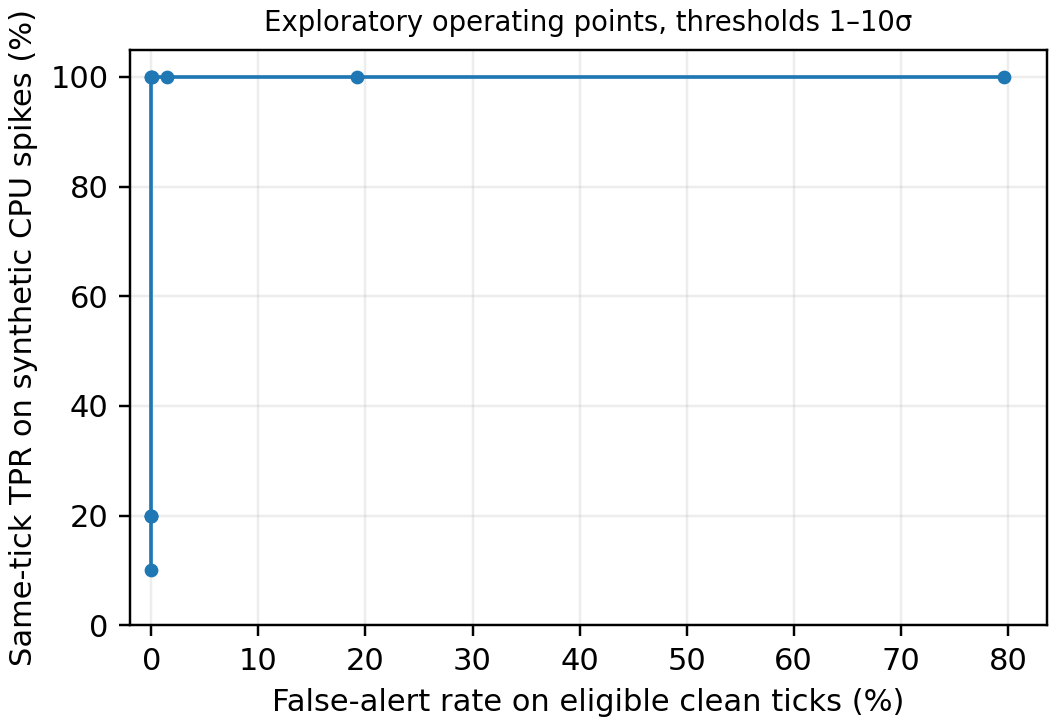
\includegraphics[width=0.78\columnwidth]{figures/seeded_roc.png}
\caption{Exploratory ROC on 300 synthetic spikes and 13,800 clean ticks across 30 seeds. Threshold-specific results are in Table~\ref{tab:seeded_roc}; coincident points have identical observed rates.}
\label{fig:seeded_roc}
\end{figure}

\begin{samepage}
The zero observed false-alert count at $k=5$ and $k=6$ applies only to these 13,800 synthetic clean ticks and is not evidence of a zero operational false-alert rate. MAD and CUSUM results and a real-attack ROC remain future experiments.
\end{samepage}

\subsection{Uniform Evaluation Rubric}
\label{subsec:rubric}

Table~\ref{tab:rubric} presents the proposed evaluation rubric; it has not yet been applied to the baseline arms.

\begin{table}[ht]
\caption{Proposed Uniform Evaluation Rubric}
\label{tab:rubric}
\centering
\setlength{\tabcolsep}{2pt}
\begin{tabular}{|p{50pt}|p{60pt}|p{75pt}|}
\hline
\textbf{Dimension} & \textbf{Metric} & {Measurement Approach} \\
\hline
Latency & P50/P95/P99 & \texttt{hdrhistogram} over instrumented paths \\
\hline
Throughput & Ops/sec & \texttt{criterion}-driven load generation \\
\hline
Fault tolerance & Recovery time & \texttt{turmoil}/\texttt{madsim} \\
\hline
Resource footprint & CPU, memory & cgroups v2 accounting \\
\hline
Data residency & Verifiable placement & Instrumented, cross-checked with OPA logs \\
\hline
DDIL degradation & Curve vs.\ loss/latency & \texttt{tc}/\texttt{netem} sweep \\
\hline
Sovereignty & Dependency count & Dependency-graph audit \\
\hline
\end{tabular}
\end{table}

\subsection{Limits of the Literature Comparison}

The source-verified implementation denominator and per-paper feature codes are pending (Table~\ref{tab:gapcounts} and the companion coding files). The documented tool capabilities in Table~\ref{tab:toolreview} are not evidence of comparative detection rates, latency or resource efficiency. Such claims require the matched evaluation described in Section~\ref{subsec:baselines}.

\section{Reproducibility Package}
\label{sec:reproducibility}

The companion working package contains the Rust source and locked dependencies, recorded unseeded run archive, seeds 0--29, synthetic trace, threshold sweep, laptop-VM latency records and SQLite log, earlier host capture, MadSim traces and weight grid, and literature working files. At its root, \texttt{make tables} rebuilds Tables~\ref{tab:rusttoolchain}, \ref{tab:ci}, and \ref{tab:rules}, replays the sigma sweep and reanalyses the saved latency and fusion outputs. \texttt{make figures} rebuilds the ROC and screening-flow plots; \texttt{make reproduce} runs both plus the statistical checks. Generated fragments are read by this manuscript.

This command reanalyses \emph{recorded} observations; it does not recreate unseeded draws, repeat VM timing, generate DDIL traffic or supply missing literature evidence. \texttt{make verify-rust} separately rebuilds seeded detector and MadSim programs and compares their outputs with the saved captures. The later K3s-pod CSV remains on the VM and is not included in this package; the displayed aggregate counts are recorded in Section~\ref{sec:production}. Raw data and run metadata must be archived before independent reproduction of that run. Paired CRANE and H1e/H1f verdicts remain unmeasured.

\section{K3s VM Pilot and Further Validation}
\label{sec:production}

On a laptop-hosted Ubuntu~24.04 VM, a single-node K3s cluster hosted test pods in which the Rust CLI and, separately, the seeded detector example were invoked with \texttt{kubectl exec}. This is the completed K3s-hosted prototype experiment. The CLI's in-memory loop ran with 500 samples and a spike every 50 ticks. Three displayed unseeded runs reported 16, 14 and 18 anomaly-bearing ticks; each reported 500 Normal ticks, zero Moderate and Strict ticks, and peak risk 45.00. These aggregate counts do not identify true or false detections. The VM test log separately showed 16 unit tests and one integration test passing.

The seeded example produced a CSV reported as 15,001 lines, including a header. The driver is configured for 30 seeds with 500 samples each. The displayed grouped counts are summarised in Table~\ref{tab:k3s_pilot}. The 198 non-spike alert-bearing ticks comprised 194 with no CPU alert and four with a CPU alert. A subsequent VM command reported 198 alert-bearing ticks among 13,800 post-warm-up non-spike ticks (1.43\%); the 14,700 non-spike total includes warm-up. Its binomial exact 95\% interval is [1.24, 1.65]\% under tick-independence, but outcomes within each seed may be dependent. This repeats the earlier 30-seed synthetic design, not 300 additional independent attack observations. The raw CSV remains on the VM; the line count and grouped output were displayed, and the post-warm-up count was reported in the session. The original and VM traces have not been compared row by row.

\begin{table}[ht]
\caption{K3s VM pilot: synthetic execution and node snapshots}
\label{tab:k3s_pilot}
\centering\footnotesize
\setlength{\tabcolsep}{3pt}
\begin{tabular}{@{}p{0.44\columnwidth}p{0.46\columnwidth}@{}}
\toprule
Measure & Observed result \\
\midrule
Seeded output & 30 configured seeds; 15,000 sample rows \\
Injected CPU spikes & 300/300 same-tick CPU alerts; 0 missed \\
Post-warm-up non-spike ticks with any alert & 198/13,800 (1.43\%) \\
Unseeded CLI alert ticks & 16, 14 and 18 in three 500-tick runs \\
CLI modes and peak risk & 500 Normal; 0 Moderate/Strict; 45.00 peak per run \\
Whole-node snapshots & 34--269~mCPU; 3,970--3,987~MiB \\
Agent latency and overhead & Not measured by this pod test \\
\bottomrule
\end{tabular}
\end{table}

Four post-run \texttt{kubectl top nodes} snapshots, captured about 15~s apart, give the whole-node ranges in Table~\ref{tab:k3s_pilot}. They include K3s and other node activity and cannot isolate LDPAD's resource use; four readings are not a sustained-load profile. These executions use in-memory synthetic metrics; they do not establish live K3s metric collection by the detector, admission control, clinical workload performance or a matched cross-platform comparison. The proposed common registry workload and labelled events remain to be run across compatible arms in Table~\ref{tab:baseline_arms}. Record the guest CPU allocation, hypervisor and K3s versions, backing storage, network, power mode and host load. A VM does not validate physical edge-device or clinical production performance.

For H1b, the planned open-loop run uses 30 recorded seeds and interleaved rates of 1, 10 and 100~requests/s over the 1--50~KiB object mix. Each rate should run for at least 60~s per seed, with failures and timeouts recorded. Report P50, P95, P99, P99.9, maximum and the measured storage-sync share, with 95\% intervals from 10,000 seed-block bootstrap resamples. At 1~request/s even this duration provides only about 1,800 requests across seeds, so P99.9 remains exploratory and longer runs may be needed. The available loopback runner does not exercise the K3s admission path or implement this full-duration schedule; both are needed for an H1b admission-path verdict. A controlled \texttt{tc}/\texttt{netem} trial and, if feasible, a real degraded mobile-data link are planned separately.

For each metric and compatible arm, simulation and VM deployment estimates will be reported separately with 95\% confidence intervals. Metrics without a valid simulated counterpart will be marked not comparable.

\noindent\textbf{Estimation and decision rule.} For each comparable metric, let $S$ and $P$ denote the simulation and deployment estimates, respectively, computed over the same scenario and, where feasible, matched seeds. The relative difference is
\begin{equation}
D = \frac{|P-S|}{|S|}\times 100\%.
\label{eq:production_gap}
\end{equation}
The point estimate meets the 20\% rule if $D\leq20\%$. The planned uncertainty analysis resamples whole matched seed pairs 10,000 times and reports a 95\% percentile bootstrap interval for $D$; individual events within a run are not treated as independent replicates. If the upper interval bound is at most 20\%, the data support agreement under this rule; if the lower bound exceeds 20\%, they do not. An interval crossing 20\% is inconclusive. If a simulation estimate or bootstrap denominator is zero, the relative comparison is not assigned a verdict and the absolute difference is reported. A simulated and deployed metric must have the same definition and measurement boundary to be compared.

Table~\ref{tab:validation_results} provides the reporting structure for the planned matched Arm~A comparison. NR refers to that comparison, not to the completed K3s test-pod result in Table~\ref{tab:k3s_pilot}. The latter used the seeded in-memory detector rather than the planned common registry workload and has no matching simulation estimate for this comparison. NR is not a measured zero; there is no basis for a 20\% agreement verdict.

\begin{table}[ht]
\caption{Arm A: Planned Matched Simulation--Deployment Agreement}
\label{tab:validation_results}
\centering
\footnotesize
\setlength{\tabcolsep}{3pt}
\begin{tabular}{@{}lrrrrl@{}}
\toprule
\textbf{Metric} & \textbf{Sim.} & \textbf{VM arm} & \textbf{$D$} & \textbf{95\% CI} & \textbf{Verdict} \\
\midrule
TPR (\%) & NR & NR & NR & NR & Pending \\
Delay (ms) & NR & NR & NR & NR & Pending \\
P99 (ms) & NR & NR & NR & NR & Pending \\
CPU (\%) & NR & NR & NR & NR & Pending \\
RAM (MiB) & NR & NR & NR & NR & Pending \\
\bottomrule
\end{tabular}
\end{table}

A future comparison evidence pack must comprise arm-specific configuration, workload and attack scripts, raw data, deployment and simulation logs, seed lists, and analysis code. No matched comparison data exist to regenerate those future tables; until the experiments and reproduction pipeline are completed, no claim of baseline superiority, clinical production equivalence, or 20\% agreement is supported.

\section{Discussion and Future Work}
\label{sec:discussion}

{RQ1:} The prototype includes seven simplified static predicates, SHA-256 drift detection, risk scoring and a 3-sigma detector over five synthetic metrics. No ablation establishes a minimum set of controls. The separate guarded fusion prototype resolves the isolated high-risk cases in the labelled scenarios but also escalates on a three-second nuisance pulse; its end-to-end performance and operational safety remain unestablished.

{RQ2:} The supplied Rust detector uses a rolling window and was executed with synthetic inputs in a K3s test pod. The four whole-node snapshots cannot establish agent-specific resource use. Continuous posture assessment and the complete agent's CPU and memory use on the target hardware remain untested.

{RQ3:} The original seeded Rust detector matched 300/300 conspicuous synthetic CPU spikes (event-level exact 95\% CI 98.78--100.00\%) and alerted on 198/13,800 eligible clean ticks (1.43\%; exact CI 1.24--1.65\%). The K3s-pod rerun reported the same aggregate spike matches and 198 alert-bearing ticks among 13,800 post-warm-up non-spike ticks (1.43\%). The CLI combines posture, drift and anomaly scores for synthetic inputs, but these repeated tests do not establish the effectiveness of the full proposed control loop, real-attack performance, operational alerts per node-day, or an advantage over another tool.

{RQ4:} The tested CLI does not include the Layer~3 local state cache or the Layer~8 reconciliation path. These are planned additions beyond the completed K3s pod run; detection integrity and recovery during partitions remain untested.

{RQ5:} The original detector component output was unresolved at integer-microsecond precision. The separate laptop-VM loopback pilot reports latency and sync share in Table~\ref{tab:latency_pilot}; its 10~request/s P99 upper confidence bound exceeded 50~ms. The K3s admission-path H1b verdict and complete-agent CPU and RAM overhead remain unmeasured.

{Limitations.} Detector and fusion results use synthetic inputs; the latency and K3s-pod pilots used a laptop VM. A resource-limited VM does not establish performance on a physical constrained edge device or in clinical production. The K3s-pod CSV and environment record have not yet been archived with this paper. The fusion experiment uses fixed, author-labelled risk vectors; its floor thresholds were chosen for the same design requirements, and its guarded fast path can falsely escalate on a brief nuisance pulse. It does not couple the detector to policy enforcement or establish independent attack accuracy. The Rust detector uses conspicuous synthetic CPU spikes and Gaussian background streams, not a deployed registry or real attacks; its event-level exact interval assumes Bernoulli outcomes, while event outcomes are grouped within 30 seeds. The separate all-events-detected-per-seed interval is a different endpoint and should not be interpreted as TPR. The short synthetic trace has no elapsed-time cadence, so no operational alerts-per-node-day rate or wall-clock detection delay is available. The 1--10 sigma sweep reuses the same trace and is exploratory; MAD and CUSUM comparators were not run. The open-loop latency pilot is a short-burst loopback experiment and does not measure the deployed K3s path. The proposed platform and tool baselines have not been compared, and no VM deployment--simulation agreement has been established. The 25-paper inventory and its coding require source verification and may not cover all relevant literature. The existing experiments do not establish comparative security effectiveness.

\textbf{Future work.} Independently label and test sustained attacks and transient benign signals, assess the fast path's false-escalation and recovery costs, and connect it to the detector and policy adapter. Complete the laptop-VM/K3s admission-to-oplog path and DDIL trial; collect a timestamped seven-day clean trace and real labelled cryptominer, bulk-read and credential-stuffing events with at least 100 episodes per event cell; compare the detector with pre-specified MAD and CUSUM baselines; repeat the threshold sweep on held-out traces; extend the simulator to network and fault injection; integrate AES-256-GCM encryption and measure its cost on the VM; and pursue a rural-clinic pilot for field validation.

\section{Conclusion}
\label{sec:conclusion}

This paper presents Rust LDPAD prototype components for K3s edge nodes in resource-constrained healthcare environments. The prototype and seeded detector were executed in a K3s test pod on an Ubuntu VM. The seeded pod run reported 300/300 synthetic CPU-spike matches and 198 alert-bearing ticks among 13,800 post-warm-up non-spike ticks (1.43\%); 198/498 alert-bearing ticks were non-spike ticks (39.8\%). An earlier x86\_64 run of the same seeded design gave the same aggregate counts. Its event-level exact 95\% interval was 98.78--100.00\% and the clean-tick interval was 1.24--1.65\%, both under independence assumptions. The separate 30/30 seed-run interval is 88.43--100.00\% and is not an event-level TPR interval. No tick cadence was recorded, so elapsed delay and alerts per node-day are unknown, and H1a across real attacks and DDIL conditions is not established. The guarded fusion prototype reached Strict in the sustained runtime scenario but also escalated on a three-second nuisance pulse. The separate loopback pilot had a 10~request/s P99 upper bound of 56.075~ms and a maximum of 143.758~ms. Real-attack validation, platform comparisons, continuous K3s monitoring, admission-path latency and agent CPU/RAM overhead remain outstanding.

\section*{Acknowledgment}

OpenAI ChatGPT helped revise portions of Sections~II--VIII and the Conclusion, and helped create companion Rust and Python evaluation code, scenarios and prospective analysis plans. DeepSeek-V3 was used for search-string suggestions and LaTeX debugging.

\appendices

\section{Literature Evidence Files}
\label{app:litmatrix}

The 25-reference inventory and coding records are provided in the accompanying literature files. Unverified decisions do not establish that a feature is absent. The original coding decisions and supporting quotations are unavailable; \texttt{literature/coding.csv} records the outstanding cells. The evidence files and count table are described in Section~\ref{sec:reproducibility}.

\noindent\textbf{Per-cell source excerpts.}
No criterion cells have yet been evidence-coded in the supplied files.


\section{Reproduction Output}
\label{app:reproduce}

This appendix presents standard-output excerpts from one of the 30 unseeded Rust CLI runs and the separate component latency command on the x86\_64 host. The CLI labels its in-memory component loop ``End-to-End Experiment''; this earlier host run did not exercise the Kubernetes admission or registry path. The later K3s-pod execution is reported in Section~\ref{sec:production}. The original linear-only CLI has fixed 100 drift risk and a capped anomaly score, explaining the 45.00 peak and zero escalations. The guarded prototype's distinct simulation log is reported in Section~\ref{subsec:fusion_eval}. The earlier host logs and seeded trace are in the companion evidence package; the later K3s CSV remains on the VM. Individual CLI alert counts are not matched true-positive counts.

\begingroup
\scriptsize
\begin{verbatim}
=== LDPAD End-to-End Experiment ===
iterations : 500
spike_every: 50
static rules evaluated : 7
static risk            : 0.00

--- Results ---
anomalies detected : 17
normal ticks       : 500
moderate ticks     : 0
strict ticks       : 0
peak unified risk  : 45.00

=== Latency Microbenchmark (AnomalyDetector::observe) ===
samples   : 100000
p50 (us)  : 0
p95 (us)  : 0
p99 (us)  : 0
\end{verbatim}
\endgroup

The following excerpt is generated from the separate guarded fusion simulation. Times are relative to the start of each synthetic scenario.

\begingroup
\scriptsize
% BEGIN GENERATED FUSION TRANSITIONS
\begin{verbatim}
Guarded fusion (simulated seconds):
Sustained runtime:
   303  Normal -> Strict (fast path)
  1950  Strict -> Moderate (dwell)
  2070  Moderate -> Normal (dwell)
3-second nuisance pulse:
   603  Normal -> Strict (fast path)
   750  Strict -> Moderate (dwell)
   870  Moderate -> Normal (dwell)
\end{verbatim}

% END GENERATED FUSION TRANSITIONS
\endgroup

\begin{thebibliography}{00}

\bibitem{b1} R. L., S. J., S. D., and I. K., ``Security in Healthcare: Enhancing the Safety of Data with Cyber Security,'' in \emph{2025 10th Int. Conf. Commun. Electron. Syst. (ICCES)}, 2025, pp. 1836--1841.

\bibitem{b2} K. Yadav, P. Suman, R. Sille, T. Choudhury, and B. L. Sahu, ``Security in Healthcare: Protecting Sensitive Patient Data,'' in \emph{2026 Intell. Bus. Ind. (IBI)}, 2026, pp. 1--8.

\bibitem{b3} Affrose, P. Lata, B. Swetha, B. N. Rao, and G. C. Reddy, ``An Effective Investigation on Health Cloud Based IoT Based Virtual Health Monitoring System,'' in \emph{2024 9th Int. Conf. Commun. Electron. Syst. (ICCES)}, 2024, pp. 539--545, doi: \href{https://doi.org/10.1109/ICCES63552.2024.10859510}{10.1109/ICCES63552.2024.10859510}.

\bibitem{b4} H. H. Bin Suhaimi and H. T. Zubair, ``Data Leakage Detection in Cloud Computing Environment,'' in \emph{2024 1st Int. Conf. Cyber Security and Computing (CyberComp)}, 2024, pp. 7--12.

\bibitem{b5} L. Ali, D. Ganesh V., N. T. J., R. Almajed, and P. Johri, ``Intelligent Security Framework for Real-Time Threat Detection and Response in Cloud Networks Using Deep Reinforcement Learning and Federated Anomaly Detection,'' in \emph{2025 3rd Int. Conf. Cyber Resilience (ICCR)}, 2025, pp. 1--7.

\bibitem{b6} P. J. Gunjale, K. Sambrekar, and S. Allagi, ``Intelligent Cloud Security Model for Healthcare: Dynamic AI-Based Threat Monitoring and Compliance Assurance,'' in \emph{2026 Int. Conf. Comput. Theory Wireless Commun. (ICCTWC)}, 2026, pp. 1--5.

\bibitem{b7} R. Kande, ``Zero-Trust Healthcare Clouds: AI-Enhanced Identity, Threat Detection, and Automated Compliance Enforcement,'' in \emph{2026 Third Int. Conf. Netw. Commun. (ICNWC)}, 2026, pp. 1--7.

\bibitem{b8} R. U. Islam, C. Savaglio, and G. Fortino, ``A NDN-aided Edge-Cloud Architecture for Continuous Smart Healthcare,'' in \emph{2025 12th Int. Conf. Future Internet Things Cloud (FiCloud)}, 2025, pp. 328--333.

\bibitem{b9} R. G. S. and S. H. J., ``Ensuring Secure Healthcare Data Storage with ANFIS and CP-ABE in Cloud Computing,'' in \emph{2025 4th Int. Conf. Innovative Mech. Ind. Appl. (ICIMIA)}, 2025, pp. 810--815.

\bibitem{b10} N. Kapileswar and J. Simon, ``PrivAudit: A Federated Transformer-Driven Anomaly Detection Framework with Differential Privacy for Secure Cloud Infrastructures,'' in \emph{2025 3rd Int. Conf. Inventive Comput. Informat. (ICICI)}, 2025, pp. 563--569.

\bibitem{b11} K. Joshi, D. P. Kaur, G. S. Dewangan, B. Nune, C. Raja, and A. Nagpal, ``Secure and Privacy-Preserving Healthcare Data Management Using AI-Based Intrusion Detection Models,'' in \emph{2026 Int. Conf. Multidisciplinary Innovations Smart Sustain. Future (MISSF)}, 2026, pp. 1--6.

\bibitem{b12} P. Joshi and S. Singh, ``A Secure Threat Detection Framework for Federated Learning in Healthcare Environments,'' in \emph{2025 Int. Conf. Cybersecurity AI-Based Syst. (Cyber-AI)}, 2025, pp. 51--58.

\bibitem{b13} R. T. Dinesh Kumar, M. S., and G. K., ``Secure Medical Record Storage in Cloud using Deep Encryption,'' in \emph{2026 Int. Conf. Electron. Renewable Syst. (ICEARS)}, 2026, pp. 1437--1441.

\bibitem{b14} S. D., A. Z. A., K. A., S. P., T. SS., and A. Kumar B., ``Blockchain-Enhanced Hybrid Cloud Healthcare Data Management Solution,'' in \emph{2025 Int. Conf. Emerg. Res. Comput. Sci. (ICERCS)}, 2025, pp. 1--6.

\bibitem{b15} G. Thakre., R. Raut, and P. Verma, ``A Review on AI-Enhanced Security in Blockchain and Cloud-Based Electronic Healthcare Records Systems,'' in \emph{2025 Int. Conf. Mach. Learn. Auton. Syst. (ICMLAS)}, 2025, pp. 1214--1219.

\bibitem{b16} J. Simon and N. Kapileswar, ``Federated Deep Learning-Driven Cloud-IoT Framework for Real-Time Healthcare Monitoring and Privacy-Preserving Anomaly Detection,'' in \emph{2025 3rd Int. Conf. Self Sustainable AI Syst. (ICSSAS)}, 2025, pp. 1866--1871.

\bibitem{b17} T. K. Kota, ``Multi-Cloud Data Engineering for Scalable GenAI-Driven Medical Insurance Analytics,'' in \emph{2025 Int. Conf. Advancements Smart, Secure Intell. Comput. (ASSIC)}, 2025, pp. 1--6.

\bibitem{b18} P. Arunachalam, A. Nallathambi, Y. Uma, D. Maheswari, S. L. Srija, and Y. Vinitha, ``Applications of Technologies Powered by the Internet of Medical Things,'' in \emph{2025 IEEE Int. Conf. Blockchain Distrib. Syst. Security (ICBDS)}, 2025, pp. 1--6.

\bibitem{b19} M. R. and G. Keerthana, ``Developing IoT Healthcare Networks Based on Cloud-Based Big Data Analytics to Maximize Performance and Security,'' in \emph{2026 4th Int. Conf. Intell. Data Commun. Technol. Internet Things (IDCIoT)}, 2026, pp. 1--6.

\bibitem{b20} A. R. Abusalih Rahumath Ali, K. Saravanan, B. B. Abirami, V. S. Pandi, V. V. Aroulanandam, and S. Parthiban, ``Enhancing Cloud Security with AI,'' in \emph{2024 Int. Conf. Sustainable Commun. Netw. Appl. (ICSCNA)}, 2024, pp. 614--620.

\bibitem{b21} B. M. and K. M.V., ``Real-Time Threat Detection and Response in Cloud-Based Telemedicine Using Deep Reinforcement Learning,'' in \emph{2025 2nd Int. Conf. Comput. Data Sci. (ICCDS)}, 2025, pp. 1--6.

\bibitem{b22} G. Narsimlu, A. Padma, B. R. Sreedhar, Swatmaram, G. Deepa, and P. Suresh, ``Assessment of Artificial Intelligence in Hybrid Cloud Security Service and Future Industry,'' in \emph{2025 9th Int. Conf. Electron. Commun. Aerosp. Technol. (ICECA)}, 2025, pp. 85--91.

\bibitem{b23} R. J. Shimpi and V. Tiwari, ``Enhancing Privacy in Health IoT Using Fog Computing with Proxy Re-Encryption and Modified Whale Optimization Algorithm,'' in \emph{2025 Int. Conf. Data Sci., Agents Artif. Intell. (ICDSAAI)}, 2025, pp. 1--5.

\bibitem{b24} G. Nithyavani and G. Naga Raja, ``A Comprehensive Survey on Security and Privacy Challenges in Internet of Medical Things Applications: Deep Learning and Machine Learning Solutions, Obstacles, and Future Directions,'' \emph{IEEE Access}, vol. 13, pp. 188955--188989, 2025, doi: \href{https://doi.org/10.1109/ACCESS.2025.3588489}{10.1109/ACCESS.2025.3588489}.

\bibitem{b25} R. Katiyar, N. Thirugnanasambandan, F. Digaswala, P. Sumathi, I. Ali, and B. B. Pinky, ``Application of AI-Driven Techniques for Smart Healthcare Monitoring Systems,'' in \emph{2026 6th Int. Conf. Inventive Comput. Inf. Technol. (ICICIT)}, 2026, pp. 1774--1778.

\bibitem{b_crane} E. Bainomugisha and A. Mwotil, ``Crane Cloud: A resilient multi-cloud service abstraction layer for resource-constrained settings,'' \emph{Development Engineering}, vol.~7, 100102, 2022, doi: \href{https://doi.org/10.1016/j.deveng.2022.100102}{10.1016/j.deveng.2022.100102}.

\bibitem{b_k3s_requirements} K3s, ``Requirements.'' [Online]. Available: \url{https://docs.k3s.io/installation/requirements}

\bibitem{b_madsim} MadSim contributors, ``MadSim: Deterministic Simulator for Distributed Systems,'' version 0.2.34. [Online]. Available: \url{https://github.com/madsim-rs/madsim}

\bibitem{b_latency_sqlite} SQLite Consortium, ``Write-Ahead Logging.'' [Online]. Available: \url{https://www.sqlite.org/wal.html}

\bibitem{b_latency_hdr} HdrHistogram contributors, ``Histogram: record\_correct,'' \emph{Rust crate documentation}. [Online]. Available: \url{https://docs.rs/hdrhistogram/7.6.0/hdrhistogram/struct.Histogram.html#method.record_correct}

\bibitem{b_prisma} M. J. Page \textit{et al.}, ``The PRISMA 2020 statement: an updated guideline for reporting systematic reviews,'' \emph{BMJ}, vol. 372, n71, 2021, doi: \href{https://doi.org/10.1136/bmj.n71}{10.1136/bmj.n71}.

\bibitem{b_falco} Falco Project, ``The Falco Project.'' [Online]. Available: \url{https://falco.org/docs/}

\bibitem{b_kubescape} Kubescape, ``The Kubescape operator.'' [Online]. Available: \url{https://kubescape.io/docs/operator/}

\bibitem{b_kubescape_runtime} Kubescape, ``Runtime threat detection.'' [Online]. Available: \url{https://kubescape.io/docs/operator/runtime-threat-detection/}

\bibitem{b_gatekeeper} Gatekeeper, ``How to use Gatekeeper.'' [Online]. Available: \url{https://open-policy-agent.github.io/gatekeeper/website/docs/howto/}

\bibitem{b_tost} D. J. Schuirmann, ``A comparison of the two one-sided tests procedure and the power approach for assessing the equivalence of average bioavailability,'' \emph{J. Pharmacokinet. Biopharm.}, vol. 15, pp. 657--680, 1987, doi: \href{https://doi.org/10.1007/BF01068419}{10.1007/BF01068419}.

\bibitem{b_netem} Linux, ``tc-netem(8): network emulator.'' [Online]. Available: \url{https://man7.org/linux/man-pages/man8/tc-netem.8.html}

\bibitem{b_ed25519} S. Josefsson and I. Liusvaara, ``Edwards-Curve Digital Signature Algorithm (EdDSA),'' RFC 8032, Jan. 2017, doi: \href{https://doi.org/10.17487/RFC8032}{10.17487/RFC8032}.
\bibitem{b_aes_wrap} J. Schaad and R. Housley, ``Advanced Encryption Standard (AES) Key Wrap Algorithm,'' RFC 3394, Sep. 2002, doi: \href{https://doi.org/10.17487/RFC3394}{10.17487/RFC3394}.
\bibitem{b_gcm} M. Dworkin, ``Recommendation for Block Cipher Modes of Operation: Galois/Counter Mode (GCM) and GMAC,'' NIST SP 800-38D, 2007, doi: \href{https://doi.org/10.6028/NIST.SP.800-38D}{10.6028/NIST.SP.800-38D}.
\bibitem{b_ct} B. Laurie, E. Messeri, and R. Stradling, ``Certificate Transparency Version 2.0,'' RFC 9162, Dec. 2021, doi: \href{https://doi.org/10.17487/RFC9162}{10.17487/RFC9162}.

\end{thebibliography}
\begin{IEEEbiography}[{
\includegraphics[width=1in,height=1.25in,clip,keepaspectratio]{developer.png}}]{Semunyu Aloyzious} received the B.S. degree in Information and Communications Technology from Gulu University, Uganda. He is currently pursuing the Postgraduate Diploma in Computer Science at Makerere University, Kampala, Uganda. His research interests include cloud security architectures, lightweight virtualization, runtime threat detection, and resource-constrained edge computing systems.
\end{IEEEbiography}
\begin{IEEEbiography}[{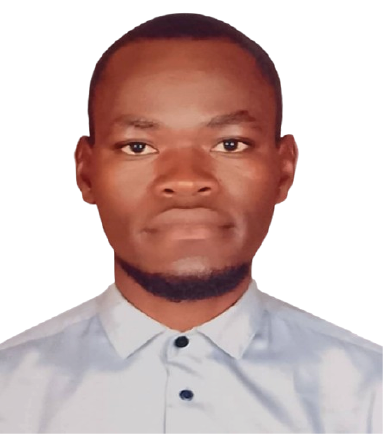
\includegraphics[width=1in,height=1.25in,clip,keepaspectratio]{stev.png}}]{Odoi Stephen} received the B.Sc. degree in Computer Science from Lira University, Uganda. He is currently pursuing the M.S. degree in Computer Science at Makerere University, Kampala, Uganda. His research interests include cloud security architectures, lightweight virtualization, runtime threat detection, and resource-constrained edge computing systems.
\end{IEEEbiography}

\EOD
\end{document}
